\chapter{Design}
\label{chapter:design}

% \epigraph{So far, we have been able to study only one evolving system and we cannot wait for interstellar flight to provide us with a second. If we want to discover generalizations about evolving systems, we will have to look at artificial ones.}{--- \textup{John Maynard Smith}}

\minitoc[n] % minitoc without title

\section{Introduction}

  \subsection{Cooperative Robots for Collective Tasks}

    \subsubsection{Multi-robots systems.} Multi-robots systems (MRS), or sometimes multi-agent robotics~\cite{Dudek1996}, essentially gained fame during 1980s under the idea of having robots cooperation in order to cope with tasks that classical single robots sometimes could not achieve. CEBOT and ACTRESS are famously often cited among the earliest successful MRS. CEBOT~\cite{Fukuda1988} (for CELlular roBOTic system) is a decentralized architecture inspired by cellular organization. The organization of the system is dynamic and robots, which are coupled to one another, can reconfigure their structure if the environment changes. This system is based on hierarchical organization where "master cells" (which are also robots) can communicate with other master cells and allocate subtasks to all the agent in the system. In comparison, in ACTRESS~\cite{Asama1989} (ACtor-based Robot and Equipments Synthetic System) the system is composed of three robots and three workstations. One of these workstations is operated by an human, one is used as image processing and the last one manages the environment. Given this heterogeneous group of six agents, the goal is for the robots to perform a purely collective task (i.e. that could not be achieved by a single robot) like pushing an object. This is particularly interesting in designing efficient communication between any level of organization.

    MRS can basically be constitued of between two to a thousand of autonomous robots~\cite{Rubenstein2014} depending on the task at hand. While it may seem counter-productive to develop and control several robots where a single robot could very well achieve the task, using a team of robots has several advantages among which~\cite{Cao1997, Arkin1998}:

    \begin{itemize}
      \item{The parallel execution of multiple robots allow the task to be achieved faster.}
      \item{Several robots can ensure robustness and reliability through \emph{redundancy}.}
      \item{It can be both cheaper and simpler to produce several simple robots that a single complex one (especially if the robot is expected to suffer destruction).}
      \item{It may be necessary to distribute several robots at the same time to achieve the task, in which case a single robot could obviously not.}
    \end{itemize}

    This implies that there are several crucial features that are often expected of MRS~\cite{Parker1994}. But it is important to note that because applications vary greatly, MRS are really different in design. This means that some of these features may not be present depending on the task at hand or the architectures adopted. First, MRS are supposed to be \emph{adaptable} and \emph{flexible}. Most often, this adaptability is found at the level of the agent, where we expect robots to react to a change in the environment and, most importantly, to a change in or induced by the other robots. This adaptability also means that, in the less decentralized systems, the control system should adapt the global organization accordingly. Then, a MRS should be \emph{robust}. This basically means that it should that the system should not be too much impacted by any failure. This is easier said than done but, as we previously said, this is also one of the main advantages of such an approach. Because robots are expected to be autonomous, it is possible to design the system so that a fault on one or several robots does not critically impact the whole system. This also means that in system such as CEBOT where some robots (in this case the "master cells") have a particular as organizers, achieving full robustness is harder and necessitates that such happening is anticipated during the design. And because MRS can be used to conduct several tasks as the same time, robots must also be able to allocate the tasks according to the actual functionning robots. Finally, it is often expected of MRS to be fully \emph{autonomous}. This means that the system as well as all the agent from which it is comprised should be able to act without human intervention. In particular, the system should be able to face the unexpected without having to wait for human control for a long time. Those features mean that MRS are most adequate in several classical robotics tasks. The most famous tasks include: foraging, object transportation, localization and mapping or path planning~\cite{Farinelli2004}.

    As we previously said, applications vary greatly. Thus there is no canonical architecture for a MRS but rather different paradigms to choose from~\cite{Cao1997, Parker2008}. First, the control of a MRS can be \emph{centralized} or \emph{decentralized}. In centralized architecture, a single agent will be responsible for controlling the system. This means that, while this agent has full knowledge other the whole system, which should theoretically allow for efficient control, this agent represents a critical point for failures. Therefore, the MRS which follow this sort of organization are rare~\cite{Parker2008} and most MRS use a decentralized approach. Decentralized architectures can be of two types: \emph{hierarchical} or \emph{distributed}~\cite{Cao1997}. In a hierarchical architecture, the system is locally centralized some agents will be in charge of a group of other agents to organize the task at hand. In comparison, in a distributed system, all agents are equal in control which, while robust, implies that it is harder to achieve coherence between every agents with relation to the task to accomplish.

    Another important design choice in term of architecture (and which is greatly relevant with relation to our problem) is on the subject of team composition: \emph{homogeneous} or \emph{heterogeneous}. In an homogeneous team, individuals are all identical in terms of both control (software) and morphological and sensory capabilities (hardware). In comparison, heterogeneous robots vary in one or the other. Most works in MRS have often been focused on homogeneous teams (TD: peut-être vérifier si récemment c'est toujours le cas) as it more practical in term of task allocation: because every agent is the same, they can all achieve the same tasks. Thus it is also more resilient to failures. In comparison, heterogeneous teams are obviously more complex in term of achieving coordination~\cite{Parker1994}. However, they can benefit from the differences between the individual to display more diverse coordinative strategies. Designing heterogenous systems rise problems which are critical in the fields of MRS~\cite{Parker2008}:

    \begin{itemize}
      \item{How to achieve efficient communications between several different robots ?~\cite{Jung2000}}
      \item{How to efficient allocate tasks between agents with differing capabilities ?~\cite{Parker2003}}
    \end{itemize}

    % À réfléchir: un bla bla sur les différentes façons de faire du task allocation et les différentes formes de communication ? Je pense pas que ça soit nécessaire mais si on a de la place... pourquoi pas ?

    \subsubsection{The origin of cooperation.} Obviously, one of the main problematics in MRS is: how to achieve cooperation ? In their popular (though now ancient) review of the field, Cao and colleagues~\cite{Cao1997} correctly deemed this as one of the research axis in MRS (alongside group architecture and resource conflicts) under the name: the origin of cooperation. We can mainly decompose this problem in two very different approaches. McFarland~\cite{McFarland1996} compared the design of collective actions in robots to a his analysis of group behaviours found in nature which he classifies in two categories (TD: vérifier que Cao ne le cite pas n'importe comment si possible): \emph{cooperative behaviour} and \emph{eusocial behaviour}. This crude classification is biologically doubtful but he was mainly basing his argument on the work of Tinbergen~\cite{Tinbergen1953}. The validity of such classification is not real importance here and does not really impact our explanation. The really interesting point here for our argument is that since nearly the beginning of MRS, people have been interested in taking inspiration from natural social behaviours for achieving coopration. Although without direct biological analogy, Parker~\cite{Parker2008} classified the design of multirobot cooperation in two similar categories: \emph{intentionally cooperative} systems and \emph{collective swarm} systems. This distinction entails different inspirations in how to ensure cooperation.

    The intentionally cooperative MRS are mostly composed of systems where agents have high knowledge of the other individuals' presence. They are capable of acting according to others' actions and capabilities and can sometimes coordinate thanks to diverse communication strategies. In this sort of MRS that McFarland said corresponds to cooperative behaviours, he deemed the agent to be selfish and to act in a cooperative fashion in order to maximize their utility. He was mostly refering to vertebrates. Under this "paradigm", there often is a very direct approach to cooperation, with a lot of emphasis and carefully designing the way robots coordinate. Moreover, this approach will often be well suited for MRS with groups of heterogeneous robots, where the origin of cooperation represents a real challenge in itself. From this it stems that this type of MRS somtimes take inspiration from distributed artificial intelligence (DAI). This field is mainly concerned with the design of distributed systems of intelligent agents~\cite{Cao1997, Panait2005} and is generally considered to be divided in two major areas of studies: distributed problem solving (DPS) and multiagent systems (MAS). To summarize quickly, DPS is mainly concerned with solving problems with several agents. As such, some of its problematics are common to MRS. For example it shares the same concern for trying to efficiently achieve task allocation between multiple agents. However, because in DPS agents are considered to always be cooperative and are usually totally disembodied, few works could contribute to MRS. In comparison, in MAS agents are often rational and, as such, are not de facto cooperators. MAS are thus interested in the collective interactions between agents, sometimes with a strong emphasis on game-theoretic approaches~\cite{Rosenschein1985}. Therefore, this has some theoretical interest for achieving cooperation in MRS. However, some have argued that MAS are not rooted enough in the physical world for them to make a powerful contribution to MRS~\cite{Cao1997, Farinelli2004}. In particular, perfect sensory information is often assumed in MAS which may render difficult direct application in robotics. For this reason, research in DAI tend to consider the mechanisms of coordinative behaviours as a black box~\cite{Parker1994}.

    % We believe selfishness is not necessarily associated with intionnally cooperation ?


    Nearly on the other end of the spectrum is collective swarm~\cite{Beni2005}, often also called collective robotics~\cite{Kube1993, Parker2008}. Although it could be argued that any MRS is a particular instance of collective robotics, we will stick here with this popular definition as to not generate confusion. In this approach, the MRS is often constituted a very high number of robots (at least several dozens) which are all simple homogeneous and distributed agents. Often also called "reactive collective robotics", agents are supposed to take inspiration from the behaviours and organization of eusocial insects and in particular from the order Hymenoptera (e.g. ants, wasps, bees) or Isoptera (e.g. termites)~\cite{Wilson1998, Werfel2014}~\footnote{More precise description of the evolution of eusocial and the altruistic behaviours of eusocial animals has been discussed in Chapter~\ref{chapter:model}. Consequently, there will not be an extensive discussion on this subject here.}. More precisely, the study of eusocial insects led to the creation of the field of Swarm Intelligence~\cite{Bonabeau1999, Zoghby2013}. This field consists of heuristics designed to solve algorithmics problems inspired by the natural behaviours found in eusocial insects. Some of the most famous algorithms that stemed from Swarm Intelligence are the ant colony optimization (ACO)~\cite{Dorigo2004a}, for which the most classical problem is to find the best travel route in traveling salesman problem, and particle swarm optimization (PSO)~\cite{Kennedy1995}, where candidate solutions to an optimization problem are thought as particles moving through the search space and interacting with other particles. The main goal of swarm robotics is to design a large colony of decentralized and self-organized robots capable of high flexibility and robustness.

    Agents in a swarm are as simple as possible and constituted of very simple sensory capabilities. In particular, direct communication between robots of a swarm is often inexistent. Instead, robots should rely on stigmergy, which means that indirect communication is achieved by observing the environment which may have been modified by another individual (e.g. the use of pheromones by ants in the natural world). Incidentally, in comparison to intentional cooperation, robots are often largely unaware of the actions and internal states of other individuals in a swarm, using rather mostly proximity information. This simplicity also means that robots are not capable of achieving much on their own and are expected to be useful only as part of the collective. In particular, the main concept of swarm robotics is that of \emph{emergence}\footnote{It is interesting to note that there are a lot of similarities in the philosophy between swarm robotics and individual-based modeling, which we touched upon in Chapter~\ref{chapter:model}. Mainly, the concept of emergence between behaviour-based agents is one that is central to IBM.}. This means that we expect to see the emergence of global collective complexity from the simple local interactions between agents of the swarm, something which is also known as \emph{self-organization}. More precisely, swarm robotics are based on the principle of superadditivity~\cite{Parker2008}, where the whole result (collective behaviour) is better than a simple sum of all the parts (the agents' behaviour). Mainly, the design process of a swarm is focused on created simple local behavioural rules that should allow the whole system to act in the desired collective way. It is as if cooperation is a side effect of individual behaviours. This is obviously tricky and time must not be critical in that case but also implies that agents are in the cheaper to produce, deploy and control. Also, because of the self-organization that stems from emergence, the tasks covered by swarm robotics often require little to no a priori assumptions. At the birth of collective robotics, this was really different to the "classical" design paradigm in robotics and especially in AI which emphasized on high reasoning and higher-levels of cognition~\cite{Bonabeau1999}. While examples of swarm robotics systems are numerous we can quickly name a couple. One of the first examples of successful swarm robotics on real robots was the \emph{Nerd Herd} by Mataric~\cite{Mataric1995}(TD: special character ?). With a group of $20$ identical robots with very simple individual capabitilies (mainly detection of obstacles and other robots) and a set of pre-programmed behaviours, he was able to create a system capable of collective behaviours of flocking, surrounding, herding and foraging. Another interisting example is that of Swarm-bot~\cite{Mondada2004, Dorigo2004, Mondada2005}. The goal was to engineer a swarm of simple identical robots capable of using self-assembly to navigate accross rough terrain and achieve different collective tasks.

    % -> This is not always that simple. Genre en swarm on peut faire plein de trucs globallement et des fois ya du knowledge (je crois). Et le swarm peut être classé en MAS (voir Panait2005)
    % -> Globalement frontière blurry encore une fois. On va assez vite parler de swarms pour des trucs qui répondent pas aux principes de base des swarms


  \subsection{The Control of Collective Robots}

    Because robots are expected to cooperate and in some case coordinate, there is a strong need for reactivity and adaptability in MRS~\cite{Iocchi2001, Farinelli2004}. The fact that multiple individuals engage in a collective behaviour implies that the individuals act in a dynamic environment. To that end, the concept of \emph{situatedness} refers to the complexity and uncertainty that exists in the environment in which the embodied robot interacts~\cite{Mataric2008}. The control of a robot mainly depends on its situatedness. In term of single robot control, several main architectures have been studied.

    First, the \emph{deliberative approach}, or sometimes also refered as the Sense-Model-Plan-Act architecture~\cite{Albus1991, Iocchi2001, Mataric2008}. This has been the classical approach in robotics~\cite{Nilsson1984} and AI for a long time because it is concerned with representing high reasoning capacities. The basic idea is that all sensory information is computed under the internal knowledge in order to plan and determine the next action. This means that these architectures are based on an internal represention of the world. This model of the world is usually constituted of a set of symboles and predicates on which logic can be applied to decide the next action. This implies that the first step of such architecture is to collect all data of the environment to build or update this model. Then, a planning phase is used to find the best possible plan given the task and finally act on this decision. Planning is a classical problem in AI and is known to be costly. Consequently, while we can understand how this architecture would be efficient in a perfect world, the process of building a world representation and planning is time consuming and lacks reactivity which is critical in real-world applications. In particular, keeping an accurate internal representation up-to-date proves to be difficult in dynamic and noisy environment.

    % Citer des architectures délibératives classiques ? (genre STRIPS ou NOAH)

    In light of the complexity of the previous architecture was born the opposite stance of \emph{reactive approach}~\cite{Brooks1986}. In comparison to a deliberate approach, this architecture is based on no reasoning nor planning. Rather, its main principle is that there is tight connection between sensors and effectors, which is inspired by the biological concept of stimulus-response. This architecture is usually constituted of a programmed set of rules which, given the sensory inputs, gives the desired output actions. This implies that this type of architecture can achieve very fast computation and thus is very convenient in situations where quick reactivity is necessary. However, as robots do not keep any representation of the world or often do not store any information which means they are basically myopic. This can be useful when a priori knowledge of the environment is sufficient but cannot deal very well with uncertainty and novelty. In particular, it cannot improve on its capacities or learn from the world.

    Then, a \emph{hybrid approach} has been proposed, whose goal was to unite the best of both worlds, namely the speed of response of reactivite approach and the optimal planning of the delibarate approach. Such architecture is basically constituted of three layers~\cite{Mataric2008}. One layer is responsible for the reaction and execution of the robot, another layer is concerned with delibaration and planning and the third and final layer which acts an intermediate between two other layers. In consequence, the main design complexity of this approach is on this last layer which is supposed to coordinate between the immediate needs that are dealed by the first layer and the more long-term decisions of the second layer.

    Finally, the last famous approach is the \emph{behaviour-based approach}~\cite{Arkin1998}. This approach was mostly created and popularized by the subsumption architecture of Rodney Brooks~\cite{Brooks1986}. This approach is sometimes closely tied with the reactive approach. In a behaviour-based architectures, the robot control in constituted of several basic behaviours, which are organised in separate modules. In a similar way as a reactive approach, these behaviours are directly connected to the sensors and will activate according to certain set of rules. However, in comparison with a purely reactive approach, these behavioural modules can keep a state or a representation of the world which allows for higher reasoning and planning. Those modules are all designed to interact with one another to collectively achieve the goals at hand. In that sense, there is a paradigm close to that of swarm behaviours. Namely, we expect global complexity to emerge from the interaction of local low-level behaviours. Behaviour-based architectures are thus efficient when the environment is dynamic and there needs to be adaptation from the robot but where pure reactivity alone is not sufficient. These architectures are usually designed by a bottom-up approach, where behaviours (which are the building blocks of the system) are added incrementally in an increasing complexity. Lastly, one principal challenge in this approach is to design the action selection, which is the process thanks to which the system will choose which behaviour choose from several~\cite{Pirjanian2000}. Two popular ways to solve this problem is either to base the selection on a prefixed hierarchy between modules or to rely on a voting mechanism.

    In the case of multi-robots systems, they can be characterized by a higher level of architecture which refers to the global control of the system in response to the dynamics of the environment. Mainly, a MRS itself can be characterized as \emph{reactive} or \emph{social deliberative} in this respect~\cite{Iocchi2001, Carpin2001}. Obviously, these concepts are very similar to the architecture of control in a single robot. In a reactive MRS, each individual deals with changes in the environment by itself without the influence of a higher control. Thus there is no particular model of the environment in the system and each agent is individually expected to cope with the changes and adapt. In comparison, in a social deliberative MRS, a global strategy will be planned so that the organization of the whole system (e.g. task allocation) can handle environmental changes. This implies that the system will come with a long-term plan to cope with these changes by using the resources available. This type of MRS may have a global representation of the world shared between the agents but it is not inevitable. It is important to note that the global architecture of the MRS may differ from that of the individuals (e.g. a social deliberative system may be composed of behaviour-based robots).

    Among all the architectures used to control each robot, the behaviour-based approach is the one used in most of the MRS~\cite{Arkin1998, Mataric2008, Parker2008}. The adaptability and simplicity of behaviour-based approaches make them the architecture choice for creating cooperative tasks and achieving coordination~\cite{Mataric1995, Iocchi2001}. For example, Parker proposed and developed the ALLIANCE architecture which she successfully implemented on real robots~\cite{Parker1994}. The main principle was to be able to design a fault-resistant system of heterogeneous robots which could coordinate to accomplish a particular task. This architecture is based on a subsumption architecture~\cite{Brooks1986} with the addition of the concepts of behaviour sets and motivations. A behavior set is composed of low-level behaviors put together to accomplish a particular task. The motivation of a set is used by the robot to know which behaviour set (i.e. action) select based for example on the fact that task is needed or on the fact that another robot is already doing the task. Then, Candea and colleagues developed the ART architecture~\cite{Candea2001} in order to design a team of robots to participate in the RoboCup competition~\cite{Kitano1997}. The RoboCup is an annual competition where teams of robots must compete in a soccer game, which requires to focus on several important challenges of MRS (e.g. collaboration, robot control, reasoning) in an adversarial context. The ART architecture in particular was composed of a team of distributed heterogeneous robots which differed both in hardware and software. These robots were able to vote on which team formation to use and then assign their role by communicating and evaluating the utility of a given role for a certain robot based on local information. Finally more recently, in an article published in Science, Werfel et al. designed independent robots capable of building a structure given by a user~\cite{Werfel2014}. They used a team of homogeneous robots, taking insperation from the mount-building capabilities of termites. These robots could communicate through stigermy (i.e. indirect communication) and followed the building rules automatically compiled from the user structure. The agents were fully reactive so that they could adapt to a change in the current structure (either from robot or human action). Given this last example, it is also interesting to quickly tell where collective robotics (i.e. swarms) stand with relation to architecture. As previously said, the similarities between reactive and the behaviour-based architectures with the paradigm of swarm behaviours are numerours. In particular, they both focus on low-level, local and individual rules so that a global collective and complex behaviour can emerge, which ensures robustness and quick decision making. For these reasons, all collective robotics architecture, when they are not automatically designed (which we will touch upon next), are always behaviour-based~\cite{Brambilla2012, Zoghby2013}.


  \subsection{Learning to Cooperate}
  \label{subsection:RL}

    In the previous subsections, we presented various architectures, both individual and global, that could be used to control a MRS. However, in the examples we presented, the systems were carefully designed with ingenious techniques so that the could perform the way it was intended. For example, the work of Werfel and colleagues~\cite{Werfel2014}, while remarkable and interesting for the scientific and engineering questions it raises, rest upon clever design rules. The system was designed so that robots could dynamically adapt to changes in the environment and still be able to perform the task at hand. However, this sort of robot design is not always easy, especially in the case of MRS where we sometimes expect some collective behaviour to emerge from the cooperation of individuals. Furthermore, this sort of systems may not fare well when facing uncertainty and changing environmental conditions. As robustness and adaptability are expect of a robot, there has been a considerable interest in developing learning methods for robotics. For example, in extension to the ALLIANCE architecture we talked about previously, Parker developed the L-ALLIANCE (for LEARNING-ALLIANCE) architecture~\cite{Parker1994}. Robots could learn form past experience and update their parameters (e.g. the propensity to choose to do a particular task) given their previous performances.

    Machine learning has always been one of the major subjects in artificial intelligence and has thus naturally been applied to the field of robotics~\cite{Hertzberg2008}. Classical machine learning can be divided into three different machine learning categories: supervised, unsupervised and reward-based. While in machine learning, the goal is generally to optimize performance (e.g. of classifiers), in mobile robotics the emphasis is more to allow the robot to adapt quickly. As such, most of the litterature about learning in robotics has been focused on reward-based techniques~\cite{Mataric2008}, most often under the term of \emph{reinforcement learning} (RL)~\cite{Sutton1998}. The main principle of RL is that a robot will learn an optimal policy (i.e. a sequence of actions depending on the states the robot is in) thanks to a value function. To put it simply, the robot will learn thanks to rewards and punishments according to its actions. In particular, RL is based on the model of markov decision processes (MDP)~\cite{Bellman1957}. To summarize quickly, a MDP is constituted of a set of states $S$ as well as a set of actions possible $A$ in each of the states. There is also a transition function $P_{a}(s,s')$ which, given a certain state $s$ and action $a$ at time $t$ represents the probability to be in state $s'$ at $t+1$. Finally, $R_{a}(s,s')$ represents the reward obtained by transitioning from $s$ to $s'$ thanks to action $a$. The goal of a MDP is to find the optimal policy $\pi$, where $\pi(s)$ indicates the action to choose in state $s$, which maximizes:

    \[
      \sum_{t=0}^{\inf} \gamma^{t}R_{a_{t}}(s_t,s_{t+1})
    \]

    where \gamma is a discount factor. In RL, the goal is generally to estimate the value function $V^{\pi}(s)$, which corresponds to the expected value of the state $s$ given that we follow the policy $\pi$ afterwards. This means that $V$ is obtained as follows:

    \[
      V^{\pi}(s)=E_{\pi}\big{\sum_{k=0}^{\inf} \gamma^k r_{t+k+1} | s_t = s \big}
    \]

    where E_{\pi} is the expected value if the agent follows the policy $\pi$. Alternatively, we also often define action-value function $Q^{\pi}(s,a)$ as the expected reward when starting from state $s$ and selecting the action $a$ and then following policy $\pi$:

    \[
      Q^{\pi}(s,a)=E_{\pi}\big{\sum_{k=0}^{\inf} \gamma^k r_{t+k+1} | s_t = s, a_t = a \big}
    \]

    As MDP nor RL are the subject of this manuscript, we will not go much more into the technical details of this technique. The last thing that is important to say here is that the main method developed in RL for robotics is that of temporal-difference (TD) learning~\cite{Sutton1988, Bradtke1996} (TODO: quand même vérifier que je dis pas trop de conneries ici). Based on the principles of TD learning, two mains algorithms have been developed: on-policy SARSA (State-Action-Reward-State-Action) and off-policy Q-learning~\cite{Watkins1989}. It is interesting to note that most RL techniques have theoretical proofs of convergence~\cite{Panait2005}. What we have presented here is but a crude summary of RL to give sufficient context to the rest of our explanation. We point those interested by the subject to more exhaustive litterature~\cite{Sutton1998, Deisenroth2011}.

    % Est-ce qu'il y a besoin d'un peu mieux expliquer où ça servirait à rien ?

    In the case of learning for multiple robots, this is obviously a bit more complicated. In particular, this means that other robots are learning at the same time or that at least the learning process must take into account the presence of other dynamic agents. Furthermore, this is against Markov's law which implies that in MDP the environment is stationary~\cite{Littman1994, Parker2008}. Consequently, directly adapting RL methods to multiple robots is not that easy. However, there exists a large litterature about learning in multiagent systems, whose theoretical and practical findings can sometimes be applied to a robotic setting~\cite{Stone2000, Yang2005, Panait2005}. 

    In MAS, two types of learning can be applied: \emph{team learning} or \emph{concurrent learning}~\cite{Panait2005}. In the case of team learning, a single learner is used and is responsible for learning the behaviours of the whole team. This does mean the team is necessarily homogeneous. In this case, as there is only a single learning, it is easier to apply techniques and algorithms from classical machine learning. However, the fact that there are multiple individuals implies this time that the learning suffers from a curse of dimensionality: the size of the states space increases with the number of agents and is complicated to take care off. This also means that learning will be centralized which may pose a problem in the case of a fully distributed MRS. 

    In comparison, in concurrent learning, every individual is an independent learner. In this case, the system face the problem we talked about previously of violating Markov law on the fact that the environment must be stationary. This means that new learning techniques must be designed before they are applied to multiple agents. In particular, other individuals are not only dynamics in the environment but are also all co-adaptating at the same time. Which means that for a particular learner, other individuals will adapt with relation to it, and himself will adapt to the fact that the other individuals adapted and so forth. In comparison to team learning, concurrent learning is faced with a particular challenge which is called \emph{credit assignment}, namely how to divide rewards. Because each individual learns independantly, there is a question and how to efficiently distribute a reward attributed depending on the whole collective's performance. There are mainly two different ways to consider credit assignment. On the one hand, it is possible to simply equally divide the team reward between every individuals, something which is known as a global reward. This means that even if there is vast differences between individuals' behaviours, all will be equally rewarded. Consequently, this may slow down the learning process as agents may not have sufficient reward feedback to improve on their strategy~\cite{Wolpert2001}. On the other hand, it is possible to adopt local rewards, where agents are rewarded based on their individual performance. However, this may lead to selfish behaviour because individuals have less incentive to help the collective. It has been shown that there may not exist a best way between global and local reward to assign credit~\cite{Balch1999}. Concurrent learning also creates a particular dynamic between learners. Because, as we said, every learner is learning at the same time, it is not find an optimal behaviour. This poses a problem which is closed to what can be found in game theory and in evolutionay game theory in particular~\cite{MaynardSmith1973, Fudenberg1998, Bloembergen2015}~\footnote{For an interested reader, evolutionary game theory has been described more complete in Chapter~\ref{chapter:model}.}. Consequently, some have been interested in the research of Nash equilibria in joint learning in MAS so as to find the best-response policies of all agents. In particular, there has been several studies on trying to apply Q-learning techniques to the realm of finding optimal policies in stochastic games~\cite{Littman1994, Claus1998, Bowling2003, Greenwald2005, Kapetanakis2005}.

    However, as big as the litterature on applying learning in MAS is, the scaling of reinforcement learning techniques in MAS to MRS still represents challenge~\cite{Yang2005}. In particular, while the results in MAS offer interesting perspectives, MRS suppose continuous actions and/or states spaces. This is something which is not that much studied in classical MAS. Also, there is the fact that robots must often act without complete knowledge of the environment or the other individuals. Information is generally incomplete in MRS~\cite{Yang2005, Fernandez2005}. To overcome these problems, and most notably the problem of continuous spaces, several different techniques have been proposed. For example Mataric focused on extracting the features from the learning space by reformulating the states and actions into conditions and behaviours~\cite{Mataric1997}. This way, the size of the spaces was greatly decreased. He also implemented shaping in order to ease the learning process by converting intermittent feedback into a continuous signal. In comparison, Fernandez and colleagues~\cite{Fernandez2005} developed a learning MRS by discretizing the states space, based on the designer's decision, and then applying an algorithm to generalize from this discrete space. This particular algorithm, called ENNC-QL, is based on a supervised approximation of the value functions. In the case of an adversarial MRS learning in a soccer context, Bowling & Veloso~\cite{Bowling2003} introduced GraWoLF (for Gradient-based WoLF). They use the policy gradient technique, which was proposed to overcome intractable and continuous states spaces~\cite{Sutton2000} as well as WoLF (Win or Learn Fast), an algorithm to converge when there is simultaneous learning. Lastly, some have been interested in applying fuzzy logic (i.e. formal logic where truth values can take any real value between $0$ and $1$) to multirobots reinforcement learning. In particular, Gultekin & Arslan~\cite{Gultekin2002} proposed a modular-fuzzy algorithm with Q-learning where fuzzy sets were used to abstract the states and actions spaces and overcome the challenge of managing the size of the spaces. Furthermore, an internal models of the agents is built and used to estimate the action of each individual. In conclusion, a copious amount of work exists in applying reinforcement learning techniques in MRS, however they need to rely on approximation and generalization algorithm in ordre to be able to cope with the size and complexity of MRS~\cite{Yang2005, Parker2008}.

  \subsection{Evolving Cooperative Robots}

    Another more recent technique for the automatic design of robots is evolutionary robotics (ER)~\cite{Nolfi2000, Doncieux2015a}. Again, as we said in Chapter~\ref{chapter:model}, we will not get here in the details of how a classical ER system functions as it was already covered in the Introduction. Rather, we want to quickly review the use of ER as a design method for engineering robots and MRS in particular. At its core, ER is the idea of applying concepts of evolutionary computation to the larger design of robots. This means using concepts of selection and variation for to create robust and adaptable robots. This should be clear after the previous Subsections that numerous techniques in robotics have been successfully inspired by biology. For example the reactive controllers are inspired from the notion stimulus-response~\cite{Brooks1986}, swarm robotics is an artificial translation of the collective behaviours of eusocial insects~\cite{Bonabeau1999} and some of the major advancements in reinforcement learning are deeply tied with the natural cognitive processes~\cite{Montague1996}. So at this point of the manuscript it should come as no surprise take inspiration from evolution as it is actually still the best example in the design of complex machines. Evolutionary robotics has been based on these concepts in order to bring an holistic approach to robotic design. The robot is considered as a whole and the evolution of its behaviour results from the interaction with the environment (and the other individuals in the case of MRS): ER works on embodied agents. In particular, few assumptions have to been made when using ER to design a robot~\cite{Bongard2013a}.

    At its core, ER can be considered as a learning technique. However, it may be risky to classify ER among learning algorithms. Indeed, while ER definitely corresponds to a learning process in the machine learning conception of the term (i.e. a process which will improve and optimize candidate solutions with relation to a goal), it is not the case in a more biological sense. In particular, there is a major difference between evolution which is a phylogenetic adaptation and learning as an ontogenetic adaptation as both work on very different time scales. Thus there sometimes seems to be a confusion between the machine learning conception of learning and that of biology. This difference becomes criticial with the recent challenges of trying to combine evolution and learning together~\cite{Urzelai2001, Mouret2014, Doncieux2015a}. We will thus be careful here to use the latter (i.e. biological) definition of learning and will generally refer to reinforcement learning in particular in this case.

    On the subject of learning, ER and RL share several similarities~\cite{Whiteson2012, Doncieux2015a}. In both techniques, the goal is for a robot to learn (or evolve) a behaviour (which is akin to a policy in RL) which maximizes a particular value: the reward in RL or the fitness in ER. ER can also be compared to the direct policy search algorithm in RL~\cite{Kober2013} because it is not focused on trying to estimate the value function of the states and actions. In comparison, it is centered on using only the global value (i.e. fitness) of a policy. Yet, when compared to RL, evolutionary robotics often implies bigger computational time in order to find a good solution. In particular, while proofs of convergence exist for RL and dynamic programming is guarantee to find an optimal policy in polynomial time~\cite{Littman1994, Whiteson2012}, ER may have to evaluate an exponential number of candidates. However, ER has also several advantages over reinforcement learning. First, ER methods can work very well under partial observability. In particular, they are not expected to follow Markov law (see previous subsection) to find a good solution. While there has been interest in studying reinforcement learning to partially observable markov decision processes~\cite{Jaakkola1994}, this means that ER may be more fit for the design of robot control in the face of uncertain environment. Then, ER is also more suited for dealing with problmes that would require continuous or a large number of states in RL (as it is the case in MRS). Again, as we previously said in the previous examples, techniques in RL exist to deal with this kind of problems. However, they often imply complex techniques in order to approximate the problem's definition so that more classical RL algorithms can be applied. In comparison, ER is at its base capable of efficiently cope with this problem. More precisely, ER explores the space of behaviours rather than that of states, which makes it a better solution when there is an explosion of the size of the states spaces~\cite{Panait2005}. Finally, evolutionary robotics does not require to define a complex representation and astate-action spaces because it is capable of directly evolving it own representation. It is also interesting to note that, because of these advantages, there is also a vast litterature (which we will not talk about here) on trying to combine tools from evolutionary computation to reinforcement learning~\cite{Whiteson2012}.

    While ER has been mainly focused on the design of single robots~\cite{Doncieux2015a}~\footnote{As the focus of this manuscript is on multirobots systems, we will not get into a detailed description of the litterature on the subject of ER for single robots. Interested readers should direct their interest towards more extensive reviews of the field~\cite{Floreano2008, Bongard2013a, Trianni2014, Doncieux2015a}.}, its potential for the engineering of complex collective systems is well known~\cite{Baldassarre2003}. As we previously said when comparing to RL, evolutionary robotics has indeed the advantage of being more easily scalables than what can be done in reinforcement learning. The design of social behaviours in ER is still new but several interesting research has been conducted in the past decades. In particular, there has been different works both on the competitive and cooperative side of social behaviours. On the competitive side, most of the work is focused on competitive co-evolution~\cite{Floreano1998, Floreano2008}. The biological inspiration behind competitive co-evolution is that several species (e.g. two in the simplest models) will be in competition for survival. This means that changes in one particular species may lead to adaptative change in the other species which again may lead the former species to adapt to these changes. In the context of evolutionary robotics, competitive co-evolution can lead to competitive improvements where both "species" are incrementally improving their behaviour in response to the improvements of that of the other species. This incremental process can give the possiblity to shape the adaptation of the robots towards more and more complexity without having to specifically design the fitness or the selection process to that end. The classical example of competitive co-evolution is that of the predator-prey model~\cite{Floreano1997}. In this model, inspired by the dynamics of the Lotka-Volterra predator-prey equations~\cite{Yorke1973}, a species of predators and a species of prey are co-evolved in the same environment. In consequence, the prey as to adapt to the predator's strategy in order to escape it and the predator has to adapt to that of the prey to be able to go on catching prey. Nolfi & Floreano studied this co-evolution problem in ER and showed that the best evolved performance for a predator strategies was the one obtained when co-evolving both the prey and the predators~\cite{Nolfi1998}. However, while these give really interisting pratical and theorical insights on the evolution of complex behaviours, work on competitive co-evolution are still few.

    In comparison, much more emphasis has been put on evolving cooperation between multiple robots. As we previously showed in this Section, there are obvious advantages of designing cooperative robots in MRS (e.g. necessity of the task, more efficient, faster execution). ER has the advantage of allowing to design automatically complex social behaviours, something that would not be easily doable by coding them directly~\cite{Baldassarre2003}. Among the more ancient examples, we can refer to the famous work of Reynolds~\cite{Reynolds1992}, creator of the "boids". He developed a simulation of artificial creatures who evolved the capabilities of coordinated group motion as well as obstacle and predator avoidance. This work had a strong biological inspiration from the collective behaviours of school of fishes. The strong ties of evolutionary robotics with biology has naturally led to applying evolution to the design of swarms~\cite{Brambilla2012, Francesca2016}. ER offers to possiblity to efficiently evolve the individual behaviours in a swarm without the tedious back and forth of between the designed individual behaviour and the desired collective behaviour. In particular, the evolution of swarms has been investigated in the Swarm-bot project~\cite{Mondada2005} from which we talked previously about. In particular, Baldassarre and colleagues~\cite{Baldassarre2007} developed an artificial algorithm capable of evolving coordination behaviours between up to $36$ connected robots. These robots negociate the common direction of motion and then get together to the desired goal even under the uncertainty of environment factors. Moreoever, they showed that the evolved robots were capable of great adaptability and generalization under various environmental conditions: number of robots, shape of the swarm, variation in the rigidity of the robots' connections, rough terrain and robots connected through a passive object. This collective behaviour only resulted from the evolution of individual behaviours, as per swarm robotics principles. On the subject of coordinated motion, Quinn et al.~\cite{Quinn2003} were among the first to evolve controllers for a cooperative task in physical robots. While they used three and as such it may be far-stretched to consider this swarm behaviour, their work had the main features of a swarm: homogeneous, distributed and emergence of a collective behaviour. Their robots were capable to perform formation-movement as well as adopting distinct roles between each others. Furthermore, the robotic agents were equiped with very limited sensory capabilities. More recently, Hauert and colleagues~\cite{Hauert2014} evolved a group of twenty simulated flying robots in the task of establishing a communication network. More precisely, they designed a task where a rescuer launch twenty autonomous robots from his position. The robots have then to coordinate to find the other rescuer and set a communication link between the two rescuers that has to been maintained up to thirty minutes. As the communication range for the rescuers and the robots is way shorter than the distance between the two rescuers, the robots have to cooperate to create the communication link. 

    In a different manner, some have been interested on the evolution of swarms with online methods. In the "classical" framework of evolutionary robotics, the evolutionary algorithm is an what we call an offline algorithm. This implies that there are two distinct phases in the development of a robot: the design phase (i.e. evolution of controllers) and the operational phase (i.e. deployment of robots)~\cite{Doncieux2015a, Francesca2016}. This makes the assumption that the environment where the robots are deployed is the same that the one where they were evoled. Or at least it is considering that the evolved controller will be sufficiently adaptable to cope with a environment conditions. In comparison, in online ER the design process is done directly in the operation environment. For multiple robots, this gave rise to distributed online evolutionary robotics, often called \emph{embodied evolution}~\cite{Ficici1999, Watson2002}. Based on this framework, Montanier & Bredeche~\cite{Montanier2011, Montanier2013} studied the evolution of altruistic cooperation. Most notably, they show the evolution of altruism in a situation of tragedy of commons~\cite{Hardin1968} and its relation with genetic relatedness and dispersion. While this work is at the frontier between model and design, it can clearly give insight into the development of cooperative robots in embodied evolution.

    Some have also been interested in the evolution of specialization (or division of labour). Specialization means that individuals will divide between several roles, either to achieve a task more efficiently or to achieve several tasks at the same time. For example, Ferrante and colleagues~\cite{Ferrante2015} have investigated the behaviours of leafcutter ants in a task were robots had to bring leaves into the nest. More precisely, robots could adopt either specialist behaviours, where some robots cut the leaves and put them into a temporary storage area and others took the leave from the storage area to get them to the nest, or a generalist behaviour (i.e. do both of the roles). They showed that they could evolve division of labour when environment conditions (the presence of a slope) made the presence of specialists more interesting.

    % Ca fait peu quand même niveau gens qui s'intéressent à division of labour. Floreano met le truc de Danesh avec les fourmis en ER. A investiguer.

    % En fait je pense qu'il faut le mettre en conclusion après ça
    Finally, to conclude this Subsection on an important point on the design of cooperative robots in evolutionary robotics. In particular, several design choices have to be made on whether the selection happens at the level of \emph{group} or that of the \emph{individual}. Also, whatever the level of selection, the groups of robots can be \emph{homogeneous} or \emph{heterogeneous}, something we already mentionned in previous Subsections. In particular, there are different advantages with relation to the evolution of cooperation with each of these choices~\cite{Waibel2009}. First, the level of selection will caracterize how the fitness will be distributed to each individuals. This is similar to the challenge of credit assignement (see Subsection~\ref{subsection:RL}). In particular, the level of selection defines if a single fitness value is given to the whole group of individuals or to each individual separately. In comparison, homogeneity and heterogeneity refers to the composition of the group. As we previously said, this choice of how to compose the group of individuals is crucial to the design of any MRS~\cite{Quinn2003}. Homogeneity will tend to facilite evaluation of the individuals as well as the emergence of cooperation: as all the individuals are similar, they all have the same interest in cooperating. In comparison, heterogeneous individuals may have conflicting needs and may act selfishly. But in return, it will be easier to evolve different behaviours as would be desired if division of labour is needed for example. While there is an interest in ER in heterogeneous teams of individuals~\cite{Lichocki2013}, in most of the research in the field, an homogeneous approach to the evolution of cooperation is taken (with generally group selection but it does not make much difference (TD: verifier ça dans le Waibel quand même)). In particular, as we saw, part of the litterature on cooperation in ER is concerned about swarm robotics which, by definition, are constituted of homogeneous individuals.


    -> Nous on fait pas du MAS: nos agents ne sont pas rationnels (Cao1997 (en gros))
          -> Mais on fait un peu du MAS quand même parce qu'on a un genre de perfect sensing
          -> Mais c'est evolutionary robotics justement pour s'écarter un peu des MAS
          -> Tout en restant en simulation. On peut avoir un argument du genre "meilleur des deux mondes". Surtout qu'il faudra avoir une discussion (rapide) sur simulation vs réel à un moment

    -> Bien justifier le fait qu'on fait du simulated robots (Nolfi en parle dans le handbook). Pourquoi on faire du vrai robot c'est chaud en ER ? Quels sont les problèmes pour passer de simul à vrais robots (reality gap) ? Et pourquoi dans notre cas on s'en fout un peu ? 
          -> Nous on s'en fout parce qu'on fait du théorique (en gros)

    Faudra dire en quoi on est différent de Potter2001 sur le premier papier (c'est du compétitif, c'est la seule différence ?)

    % !!! Quinn a dit c'est peut-être bien l'aclonal !!!






































\section{Evolution of Cooperation in Evolutionary Robotics: the Tradeoff between Evolvability and Efficiency}

  \subsection{Introduction}

  The evolution of cooperative actions in evolutionary robotics is as much a challenge as an interesting perspective for the design of complex collective systems~\cite{Doncieux2015}. As such, it has been widely studied with very diverse approaches and objectives~\cite{Waibel2009, Hauert2014, Trianni2007, Lichocki2012}. These works often use a clonal paradigm, where each robot has a copy of the same genome. This makes sense as this is the easiest way to ensure cooperation when individuals are expected to display similar behaviors. Moreover, using clones ensures minimal genetic relatedness between individuals, which is known to allow the evolution of altruism~\cite{Waibel2011, Montanier2011}. As such, most research focus on increasing the probability for the cooperative solution to evolve.

  In comparison, the nature of coordination behaviors and their influence on the quality of cooperation has yet to be thoroughly studied. In particular, interactions between clones in evolutionary robotics tend to produce homogeneous behaviors when most coordination tasks could benefit from heterogeneous behaviors. This could be solved by using a non-clonal approach where paired individuals do not use the same genome, and could possibly evolve different behaviors more easily. However, a non-clonal approach may face a \emph{chicken-and-egg} dilemma: multiple individuals need to behave in a particular fashion for cooperation to be rewarding, but no benefit can be extracted from this behavior unless all individuals cooperate. Therefore, without cooperating partners, those behaviors cannot be selected by the evolution as they do not benefit the individual. This is particularly problematic when a moderately rewarding solitary strategy overshadows a more rewarding, but also more challenging to evolve, cooperative strategy~\cite{Skyrms2004}.

  In this paper, we are interested in the comparison between clonal and non-clonal approaches on two different criteria:
 \begin{itemize}
    \item{\emph{Evolvability} of cooperation, which is the number of successful runs where cooperation evolved.}
    \item{\emph{Efficiency} of cooperation. This criteria is focused on the quality of the evolved behaviors and is determined by the   performance (w.r.t. fitness score) of the coordination strategies.}
  \end{itemize}

  To that end, we design a foraging task where both cooperative and solitary strategies are possible but where cooperation provides the largest reward. This task is favored by the evolution of efficient cooperative behaviors and we compare different approaches on both criteria. The first approach is a straightforward implementation of the literature where interacting individuals are clones. In comparison, the second approach is a rather extreme implementation of a non-clonal approach: we use coevolution, where individuals are from two different populations, and where fitness scores are computed independently for each individual. While this scheme is typical of competitive coevolution~\cite{Floreano1997, Floreano1998, Panait2005}, the nature of the task considered here makes cooperation more interesting, as both individuals can selfishly benefit from being cooperative.

  In the next section, we describehe methods and experimental setup used throughout our study. Then, we compare the results of the two approaches on the cooperative task. This first experiment reveals that both approaches face a tradeoff between evolvability and efficiency, where neither one dominates the other on both criteria. We investigate in a second experiment the possibility to overcome this tradeoff for both approache s. To this end, we use incremental evolution~\cite{Harvey1994, Urzelai1998} and evolve coordination in a simpler task in order to improve both the evolvability and efficiency on the target task for each approach. Finally, we discuss the implication of our findings in the last section, in particular with respect to maximizing evolvability and efficiency alike.


  \subsection{Methods}
  

  Two robotic agents are placed in a 800 by 800 units square arena with four solid walls and emptied from any obstacle apart from the targets in the foraging task. Each circular-shaped agent, with a diameter of 20 units, has a collection of sensors divided between a 90 degrees front camera and 12 uniformly distributed proximity sensors. The camera is composed of 12 rays with infinite range which indicate the type (coded on 3 bits) and proximity (one value in $R^n$) of the nearest object or agent in their direction. Proximity sensors have a range of twice the agent body's diameter and are used to get the distance to any obstacle nearby such as solid objects, the other agent or walls. The two agents always begin the simulation next to one another at one end of the arena, whereas all the objects' initial positions are randomized.

  Agents can move freely in the environment and are controlled by a fully connected multi-layer perceptron with a single hidden layer, the topology of which does not change during the evolution. Inputs of this neural network are fed with all the data extracted from the sensors: 48 neurons for the camera (4 neurons for each of the 12 rays) and 12 neurons for the proximity sensors. A bias neuron, whose value is always 1, brings the total number of input neurons to 61. The hidden layer is comprised of 8 neurons and the output layer of 2 neurons giving the speed of each of the agent's wheels. The activation function used is a sigmoid.

  In each experiment, individuals evolved during a fixed amount of evaluations thanks to an evolutionary algorithm. Their genome consists of a collection of the 506 connection weights (as real-values) of the neural network and is initially randomized for each individual in the population. Three evaluation setups are used to compare the different approaches of our experiment: 

  \begin{itemize}
    \item{In the \emph{control} setup, each individual is evaluated against 5 other randomly chosen individuals in the population except itself. Therefore we ensure that there is no genetic relatedness between individuals in each pair. However, it is not clear how the evolutionary algorithm itself may impact the population's diversity, especially because elitism is used;}
    \item{In the \emph{clonal} setup, each individual is evaluated once against a clone of itself. This setup is used to study the results of the classical clonal approach~\cite{Waibel2009, Hauert2014, Trianni2007, Lichocki2012}. While previous works have shown on multiple occasions that cooperation can evolve, it is not clear if individuals can take different roles during a cooperative interaction;}
    \item{In the \emph{coevolution} setup, each ofhe two individuals comes from two different coevolved populations. In this setup, each individual from one population encounters 5 random individuals from the other population. As pairing considers individuals from two seperate populations, the evolution of heterogeneous behaviors is theoretically easier. As a matter of fact, such a relation where two very different individuals find a selfish   interest in mutual cooperation is actually quite common in nature~\cite{Connor1995}.}
  \end{itemize}
 A pair of individuals then interact in the arena described before for a fixed number of simulation steps called a trial. Each trial is conducted $5$ times to account for the random initial positions of the objects and decrease the influence of the initial conditions on the individuals' performance. 
  
  The selection method used in the evolutionary algorithm is an elitist (10+10)-ES where the 10 best individuals in the population are used to generate 10 offsprings for the next generation. We use no recombination and therefore each offspring is a mutated copy of its parent. Mutations were sampled according to a gaussian operator with a standard deviation of \(1.10^{-2}\) and a gene's mutation rate of \(5.10^{-3}\). Finally, population size was kept constant through the evolution with a number of $20$ individuals. All experiments were done using the framework for evolutionary computation SFERESv2~\cite{Mouret2010}, which includes a fast 2D robotic simulator. The source code for reproducing the experiments is available for download at http://pages.isir.upmc.fr/\textasciitilde bredeche/Experiments/ECAL2015-coop.tgz.


  \subsection{Cooperative Foraging Task}
  
  In this first experiment, we investigate the evolution of cooperation in a foraging task. The environment is filled with 18 solid targets that the agents can collect. To collect a target, an agent has to stay close to this object for a fixed amount of simulation steps (800). After this duration, the target disappears and any agent close to it is rewarded with its value. Targets are of two types. Green targets always reward 50 when collected whereas purple ones reward 250 only when the agents collect it together (Table~\ref{tab:Rewards}). If a solitary agent collects a purple target, it disappears and rewards nothing. Consequently, there is both an incentive and a risk to cooperate as cooperation is dependent on successful coordination. This setup is a robotic implementation of a well-known problem in game theory for studying the evolution of mutualistic cooperation: the {\em Stag Hunt}~\cite{Skyrms2004}.

  The fitness score (\(F\)) of an individual is the average reward per trial:
 \[
  F = \frac{1}{N*M} \sum_{i=1}^{N} \sum_{j=1}^{M} f_{ij}
  \]
  
  Where \(N\) is the number of individuals encountered ($5$ in the control and coevolution setups, $1$ in the clonal setup), \(M\) the number of trials ($5$) and \(f_{ij}\) the rewards obtained at trial \(j\) with individual \(i\).

  When a target is collected, another target of the same type is then placed at a random position in the arena to keep a constant ratio between green and purple targets. Each evaluation lasted 20000 simulation steps and 60 independent runs were conducted for each experimental setup, each one lasting 40000 evaluations.

  \begin{table}[hbtp]
    \center{
      \begin{tabular}{lrc}
        \hline
        \multicolumn{2}{l}{\textbf{Target}} & \textbf{Reward} \\
        \hline
        Green & & \\
        & \textit{alone} & 50 \\
        & \textit{coop} & 50 \\
        Purple & & \\
        & \textit{alone} & 0 \\
        & \textit{coop} & 250 \\
        \hline
      \end{tabular}
    }
    \caption{Rewards for the foraging of the different targets, depending on whether they were collected alone or cooperatively.}
    \label{tab:Rewards}
  \end{table}

  \subsubsection{Results}

  \begin{table}[hbtp]
    \center{
      \begin{tabular}{lccc}
        \hline
        \textbf{Setting} & \textbf{\# Coop.} & \textbf{\# Solitary} & \textbf{Total}\\ 
        \hline
        \textit{Control} & 10 & 50 & \textbf{60}\\
        \textit{Clonal} & 28 & 32 & \textbf{60}\\
        \textit{Coevolution} & 14 & 46 & \textbf{60}\\
        \hline
      \end{tabular}
    }
    \caption{Number of simulations where the best individual evolved a cooperative strategy (collecting purple targets) or a solitary strategy (collecting green targets) for each setup in the foraging task.}
    \label{tab:ForagingCoop}
  \end{table}

  We are interested in the number of simulations where cooperation evolved (i.e. the \emph{evolvability} of each approach), which means simulations where the best individual in the population evolved the cooperative foraging of the purple targets (i.e. more than $50$\% of the collected targets are purple). Results for the three setups are displayed in Table~\ref{tab:ForagingCoop}. As could be expected from the literature, the clonal setup displays a greater evolvability w.r.t. evolving cooperation (28/60), whereas coevolution (14/60) is on par with the control setup (10/60). It is also apparent that cooperation is still difficult to evolve as in the best case (clonal), no more than half the simulations display the evolution of cooperative behaviors.

  \begin{figure}[hbtp]
    \begin{center}
      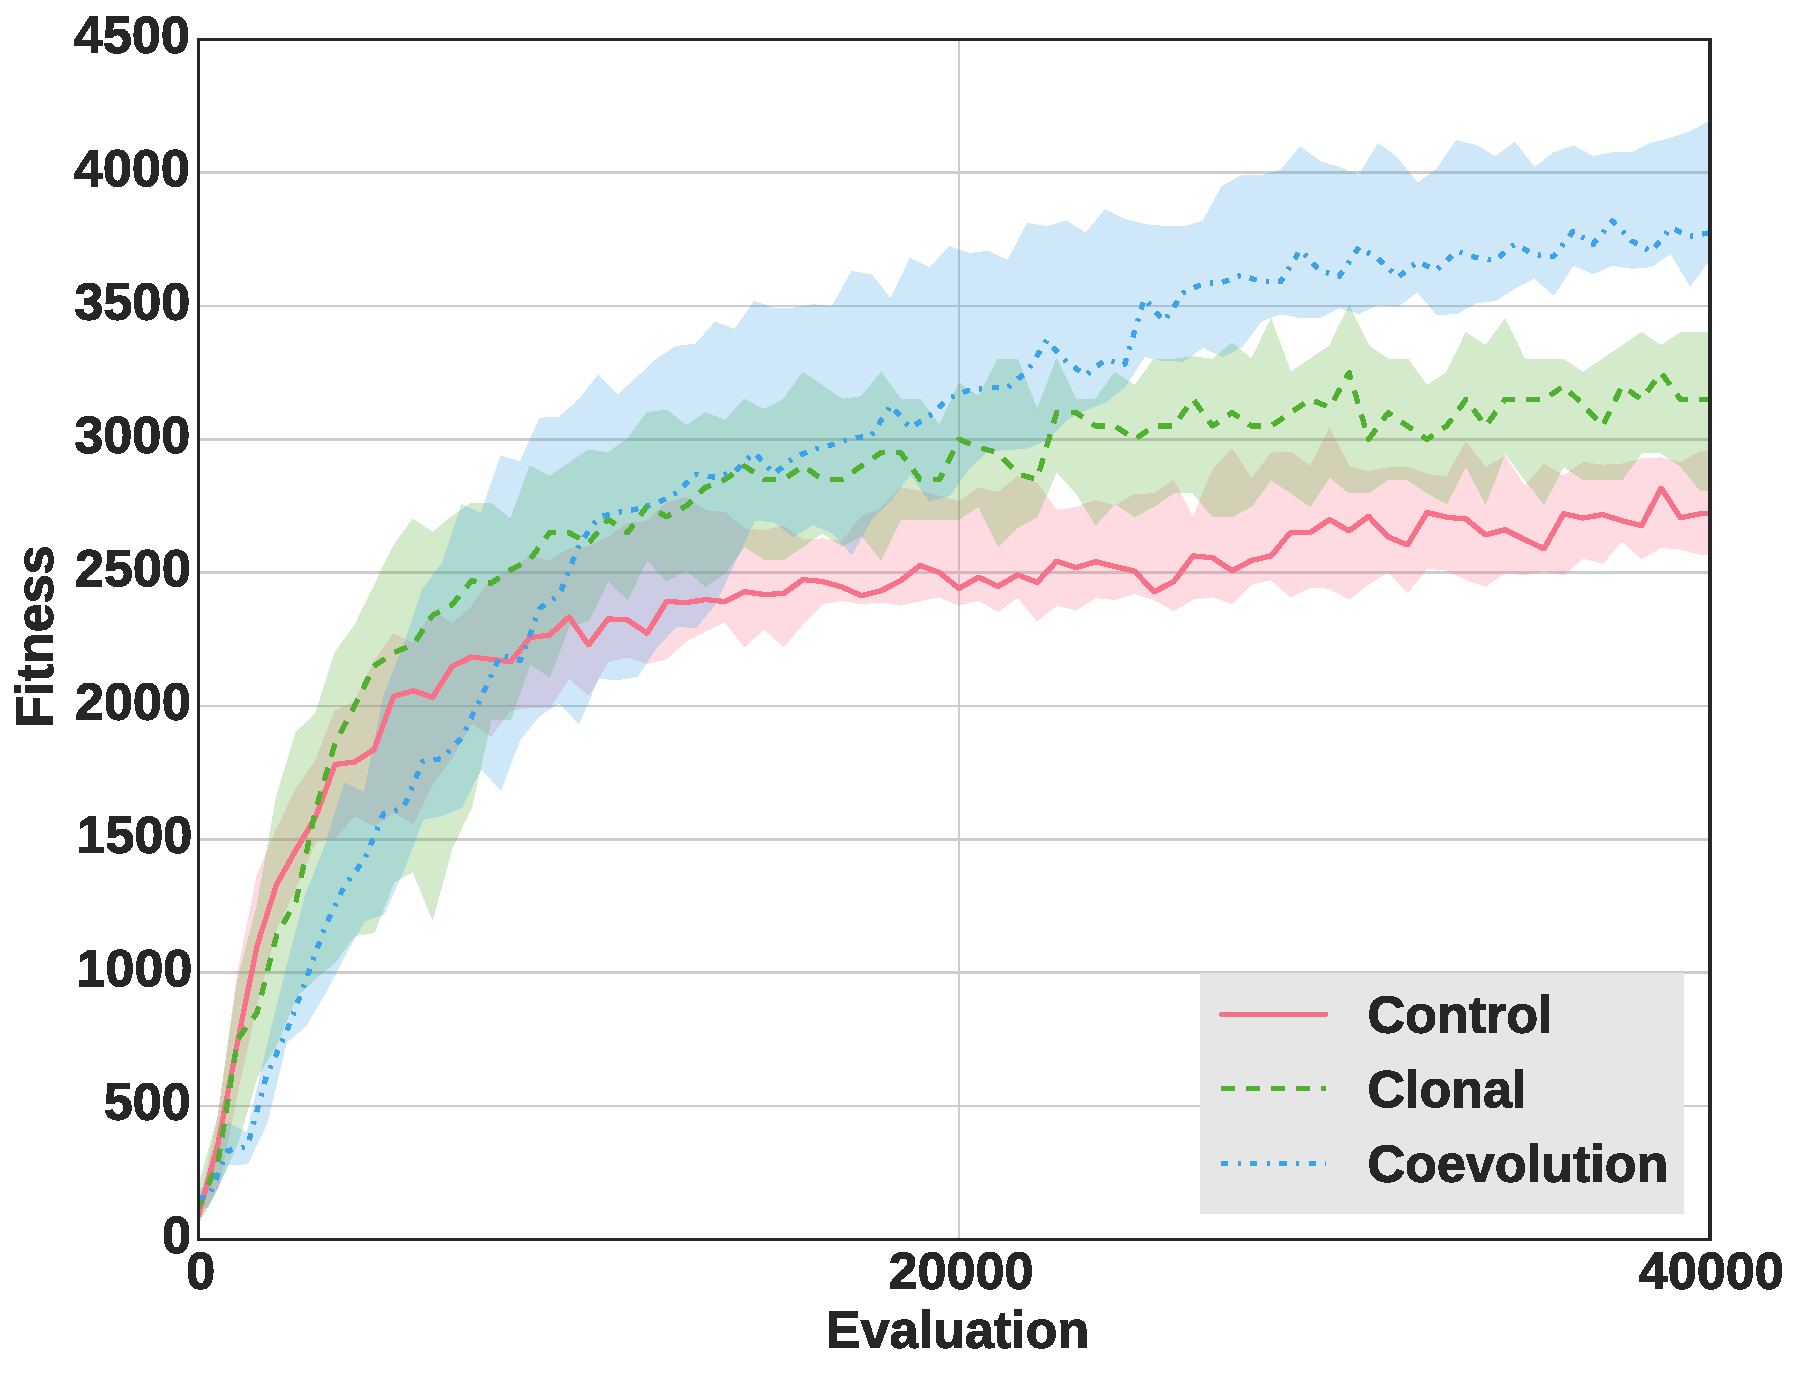
\includegraphics[scale = 0.30]{fig/ArticleRob1/fitnessHuntingStags.pdf}
      \caption{Median fitness score of the best individuals in each of the runs where cooperation evolved for each setup over time. The fitness score of an individual is computed as the average reward the individual earned per trial by foraging targets. The colored areas around the medians represent the first and third quartiles.} 
      \label{fig:HuntingFitness}
    \end{center}
  \end{figure}

  However, cooperative individuals do not perform with the same \emph{efficiency} from one setup to another. We show in Figure~\ref{fig:HuntingFitness} the median fitness score of the best individuals in each independent run where cooperation evolved over time and for each setup. Fitness scores are significantly different in each setup with the best score obtained in the coevolution setup and the worst in the control setup (Mann-Whitney U-test on the fitness score of the best individuals at the last evaluation, {\em p}-value $< 0.001$).

  These differences in efficiency can be explained by looking at the nature of the cooperative behaviors evolved, which reveals two types of behaviors: \emph{turning} and \emph{leader/follower}.

  Individuals adopting the turning strategy turn around one another so that they always see the other individual as well as stay close to it (Figure~\ref{fig:behaviorHuntingTurning}). This allows the two individuals to approach simultaneously a same target and therefore forage it in a cooperative fashion. In this strategy, both individuals have a similar behavior and no role division is necessary for their successful cooperation.

  In comparison, individuals which evolve a leader/follower strategy adopt a differentiation between two roles: \emph{leader} and \emph{follower} (Figure~\ref{fig:behaviorHuntingLeadership}). The individual we call leader always goes first on a target whereas the follower always arrives second on the same target. We observe that the follower's behavior consists in staying close to the leader and always keeping it in front of itself. In comparison the leader shows a lesser interest in the presence of its follower and rarely checks on its position.


  \begin{figure}[hbtp]
    \centering
      \begin{subfigure}[]
        {\label{fig:behaviorHuntingTurning} 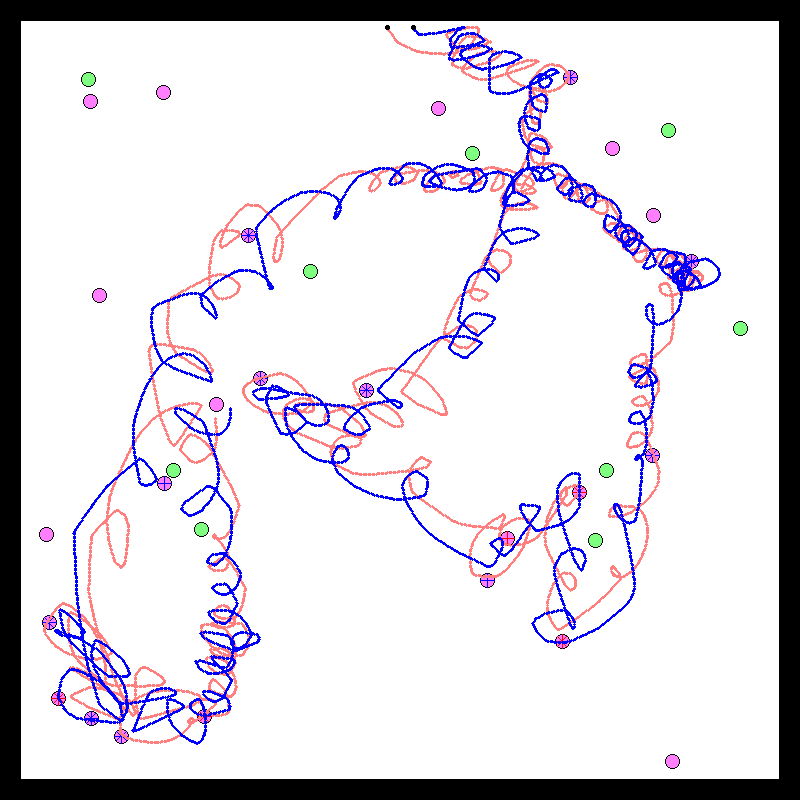
\includegraphics[scale=0.25]{fig/ArticleRob1/behaviorHuntingTurning.png}}
      \end{subfigure}~
      \begin{subfigure}[]
        {\label{fig:behaviorHuntingLeadership} 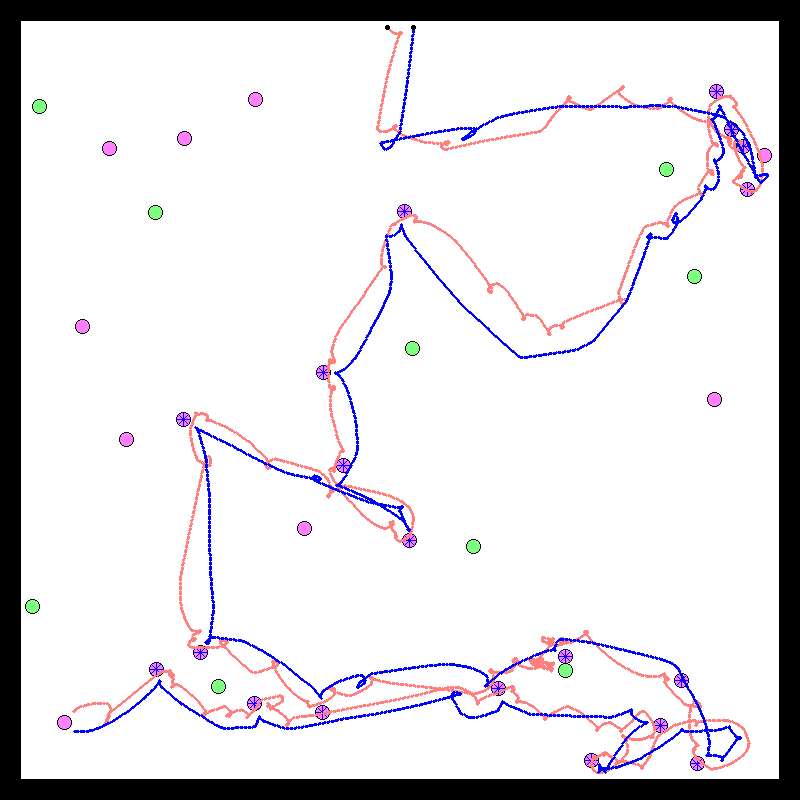
\includegraphics[scale=0.25]{fig/ArticleRob1/behaviorHuntingLeadership.png}}
      \end{subfigure}
      \caption{Snapshots of the simulation after an entire trial in the foraging task. The path of each robotic agent from their initial positions (black dots) is represented in red and blue. The green and purple discs represent the 18 targets in the environment. When a target is foraged by the two agents, a red cross (resp. blue) is drawn on the target if the red agent (resp. blue) arrived on it first. Each snapshot corresponds to a trial where agents adopted a different behavior: {\em (a)}~turning or {\em (b)}~leader/follower.}
      \label{fig:behaviorTracesHunting}
  \end{figure}


  Table~\ref{tab:ForagingBehaviors} shows the distribution of cooperative strategies for all three setups. Whereas the control and clonal setups always resulted in turning strategies (resp. 10/10 and 28/28), the coevolution setup always displayed the evolution of a leader/follower strategy (14). We observe that this latter strategy leads to more efficient cooperation. Indeed, individuals adopting the turning strategy are forced to check constantly on the other individual's position. Consequently, they cannot be as fast as individuals with a leader/follower strategy where they move to the target in a straight line under the leader's direction. Moreover, due to the random proximity of the targets, the turning strategy is prone to errors. Namely, they often get to another target than that of their partner whenever two targets are too close to each other.

  A possible explanation as to why no leader/follower strategy could evolve in the control and clonal setups may be because of the need to differentiate between the two roles. Indeed, there needs to be the existence of an asymmetry between the two individuals for this phenomenon to appear. With coevolved populations, this asymmetry is deliberately created by the separation between the two populations. Indeed, we observe that one population exclusively contains leaders while the other exclusively contains followers. 

  The two other setups fail to evolve heterogeneous behaviors. In the control setup, this may be due to the evolutionary algorithm used, especially with elistism enforcing the homogenization of the population throughout the course of evolution (as hinted in the Methods Section). Then, the clonal setup introduces yet another challenge as switching to a particular role can only be done during evaluation as both individuals are by definition genetically similar.

  \begin{table}[hbtp]
    \center{
      \begin{tabular}{lccc}
        \hline
        \textbf{Setting} & \textbf{\# Leader/Follower} & \textbf{\# Turning} & \textbf{Total}\\ 
         & \textbf{Strategy} & \textbf{Strategy} & \\ 
        \hline
        \textit{Control} & 0 & 10 & \textbf{10}\\
        \textit{Clonal} & 0 & 28 & \textbf{28}\\
        \textit{Coevolution} & 14 & 0 & \textbf{14}\\
        \hline
      \end{tabular}
    }
    \caption{Repartition of the different strategies evolved in each of the runs where cooperation evolved for each setup in the foraging task. We indicate in each cell the number of simulations where a particular strategy evolved.}
    \label{tab:ForagingBehaviors}
  \end{table}

  \subsection{Going Beyond the Evolvability vs. Efficiency Tradeoff using Incremental Evolution}

  The previous section revealed a tradeoff between evolvability and efficiency. In the clonal setup, cooperation evolves more often than with other setups. However, the coevolution setup yields cooperative behaviors which are more efficient, with paired individuals displaying asymmetrical behaviors.

  In this section, we address the following question: is it possible to benefit from both evolvability \textit{and} efficiency with the clonal and/or the coevolution setups? In other words, we explore (1) whether the clonal setup can be used to evolve pairs with heterogeneous behaviors, and (2) whether the coevolution setup can be improved in terms of number of runs where cooperation evolved.

  In order to address this question, we use incremental evolution, a rather common method in evolutionary robotics for solving challenging problems~\cite{Dorigo1994,Saksida1997,Bongard2008,Doncieux2013}. The main principle is to ease the learning of a complex task by splitting it into simpler sub-tasks~\cite{Perkins1996}.

  In the following, we introce an additional task, the \textit{waypoints crossing} task, which requires the evolution of coordination behaviors, and is simpler to address than the preous task. Individuals evolved in this first task are then used as starting point for the original task described earlier, hoping that cooperative behavior will be \emph{recycled} from the first task to the second task.
  
  \subsubsection{Waypoints Crossing Task}  

  We consider a task where robotic agents have to cross randomly positioned waypoints. As such, these round waypoints do not act as obstacles and have a diameter of 30 units. As soon as an agent goes through a waypoint, it can not be seen by this agent anymore. All 18 waypoints have the same color and can be crossed in any order. The fitness score (\(F\)) of each individual is defined as the average longest sequence of waypoints shared by both agents per trial:

  \[
  F = \frac{1}{N*M} \sum_{i=1}^{N} \sum_{j=1}^{M} l_{max_{ij}}
  \]

  Where \(N\) is the number of individuals encountered ($5$ in the control and coevolution setups, $1$ in the clonal setup), \(M\) the number of trials ($5$) and \(l_{max_{ij}}\) the longest sequence of waypoints shared by both individuals at trial \(j\) with individual \(i\).

  This implies that the two individuals are rewarded when crossing waypoints in the same order as well as maximizing the number of waypoints crossed. Each evaluation lasted $10000$ simulation steps and $60$ independent runs were conducted for each experimental setup, each one lasting $40000$ evaluations.

  \begin{figure}[hbtp]
    \begin{center}
      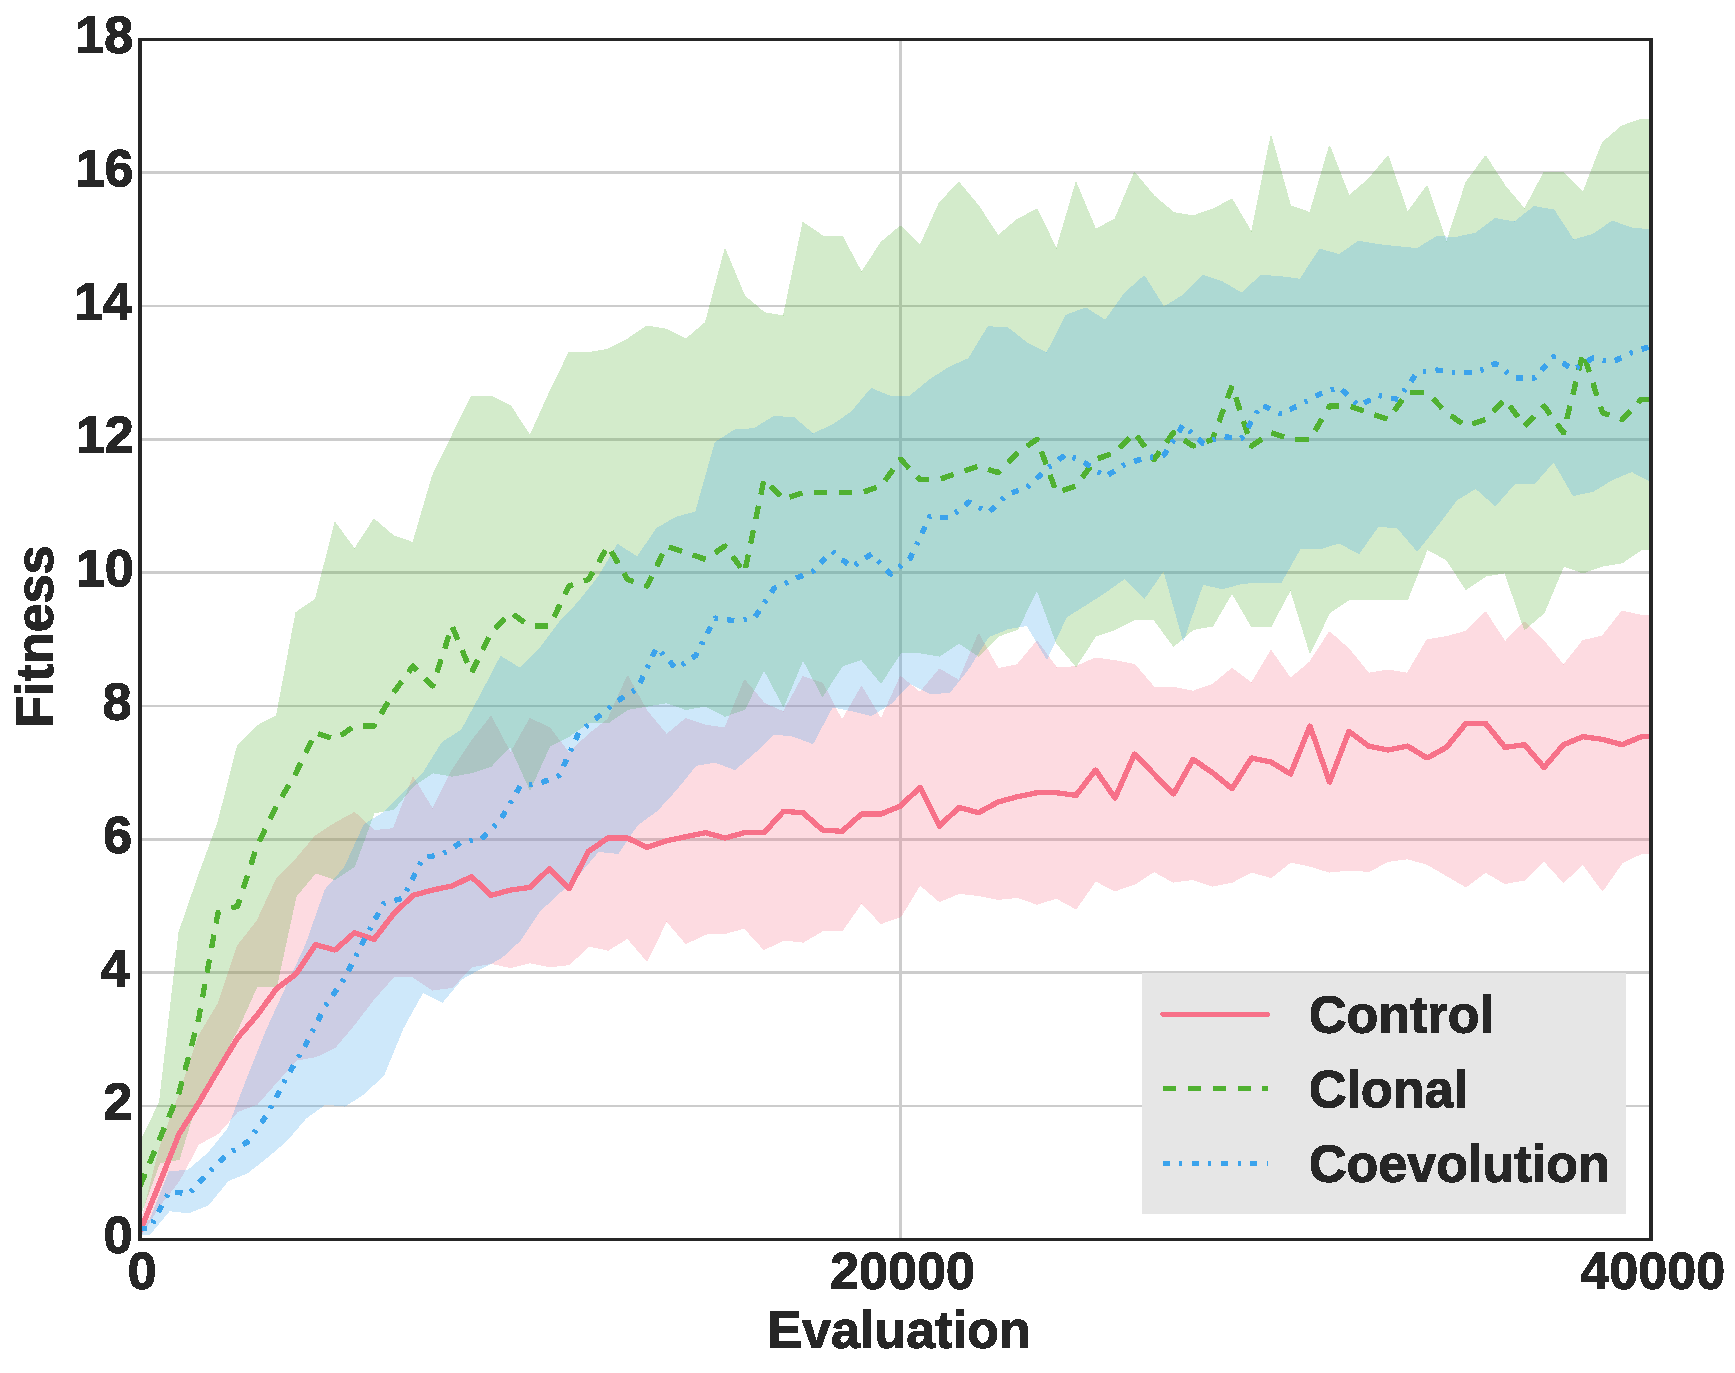
\includegraphics[scale = 0.3]{fig/ArticleRob1/fitnessWaypoints.pdf}
      \caption{Median fitness score of the best individuals in each of the 60 independent runs and for each setup over time. Fitness score is computed as the average longest sequence of waypoints shared by both agents per trial. The colored areas around the medians represent the first and third quartiles.}
      \label{fig:WaypointsFitness}
    \end{center}
  \end{figure}

  All simulations showed an increase in fitness score for each of the three setups (cf. Figure~\ref{fig:WaypointsFitness}). This was expected as this task does not represent a particular challenge for the individuals: it simply needs the evolution of a successful coordination strategy. However, whereas the coevolution and clonal setups performed equally, they both surpassed the performance of individuals from the control setup (Mann-Whitney, {\em p}-value $< 0.001$).

  As with the previous foraging task, we can hypothesize that these differences in fitness scores are due to differences in the behaviors evolved. Table~\ref{tab:WaypointsBehaviors} gives a classification of the cooperative behaviors for each setup. They are similar to those in the previous task with the addition of a third rare strategy: the \emph{wall-following} strategy (which is regrouped in ``Other''). Wall-followers simply follow the walls around the arena and cross any waypoints close to the wall they are adjacent to. As such, this is a far less efficient strategy than the two others. 


  \begin{table}[hbtp]
    \center{
      \begin{tabular}{lcccc}
        \hline
        \textbf{Setting} & \textbf{\# Lead.} & \textbf{\# Turn.} & \textbf{\# Other} & \textbf{Total}\\ 
         % & \textbf{Strategy} & \textbf{Strategy} & \textbf{Strategy} & \\ 
        \hline
        \textit{Control} & 19 & 37 & 4 & \textbf{60}\\
        \textit{Clonal} & 23 & 31 & 6 & \textbf{60}\\
        \textit{Coevolution} & 59 & 1 & 0 & \textbf{60}\\
        \hline
      \end{tabular}
    }
    \caption{Repartition of the different strategies evolved in each of the 60 independent runs for each setup in the waypoints task. We indicate in each cell the number of simulations where a particular strategy evolved: \emph{Leader/follower} (Lead.), \emph{Turning} (Turn.) or \emph{Other}. ``Other'' regroups wall-following strategies or simulations where no recognizable strategy evolved.}
    \label{tab:WaypointsBehaviors}
  \end{table}

  \begin{figure}[hbtp]
    \centering
      \begin{subfigure}[]
        {\label{fig:leadershipControl} 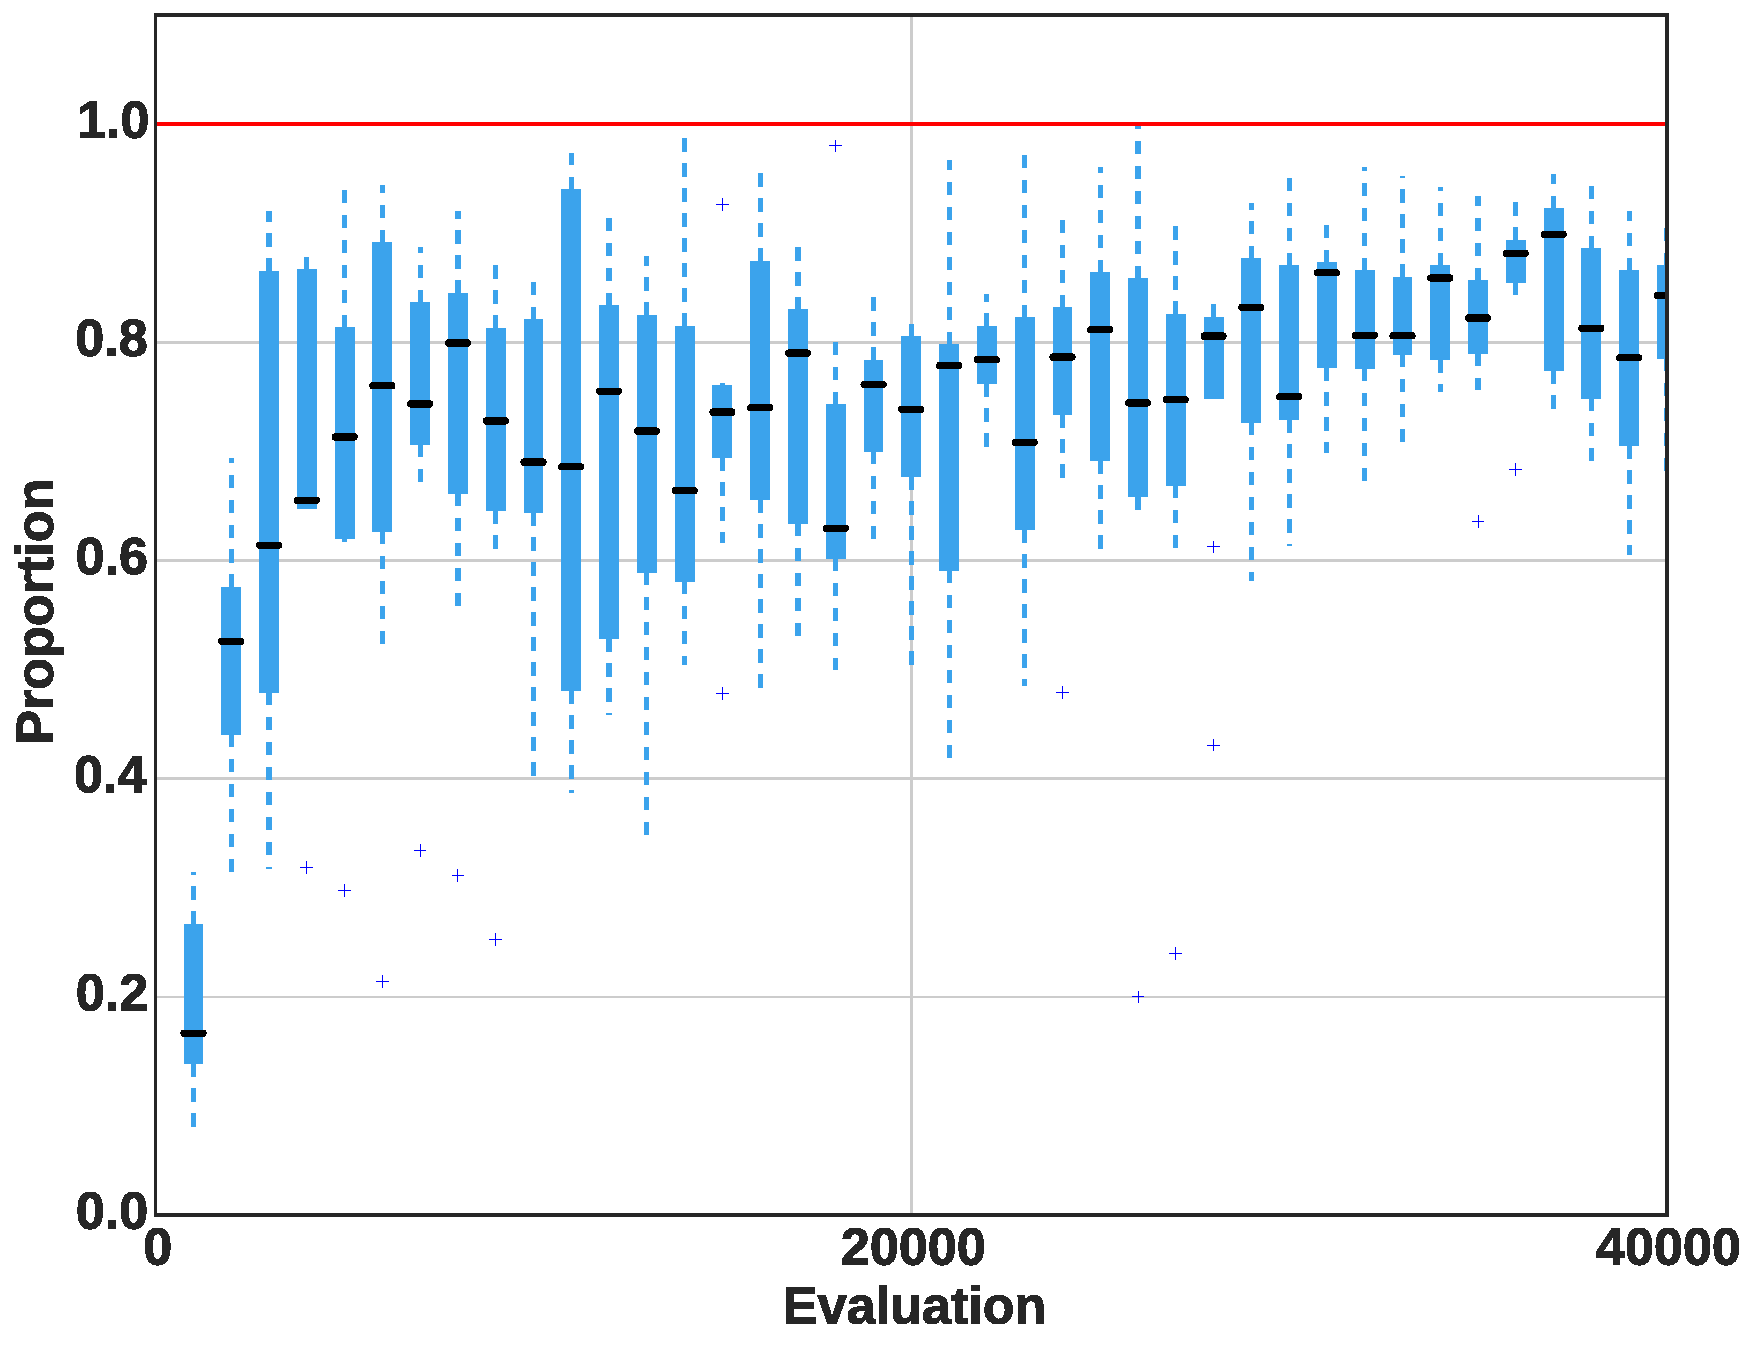
\includegraphics[scale=0.19]{fig/ArticleRob1/proportionLeadershipControl.pdf}}
      \end{subfigure}
      \begin{subfigure}[]
        {\label{fig:leadershipClonal} 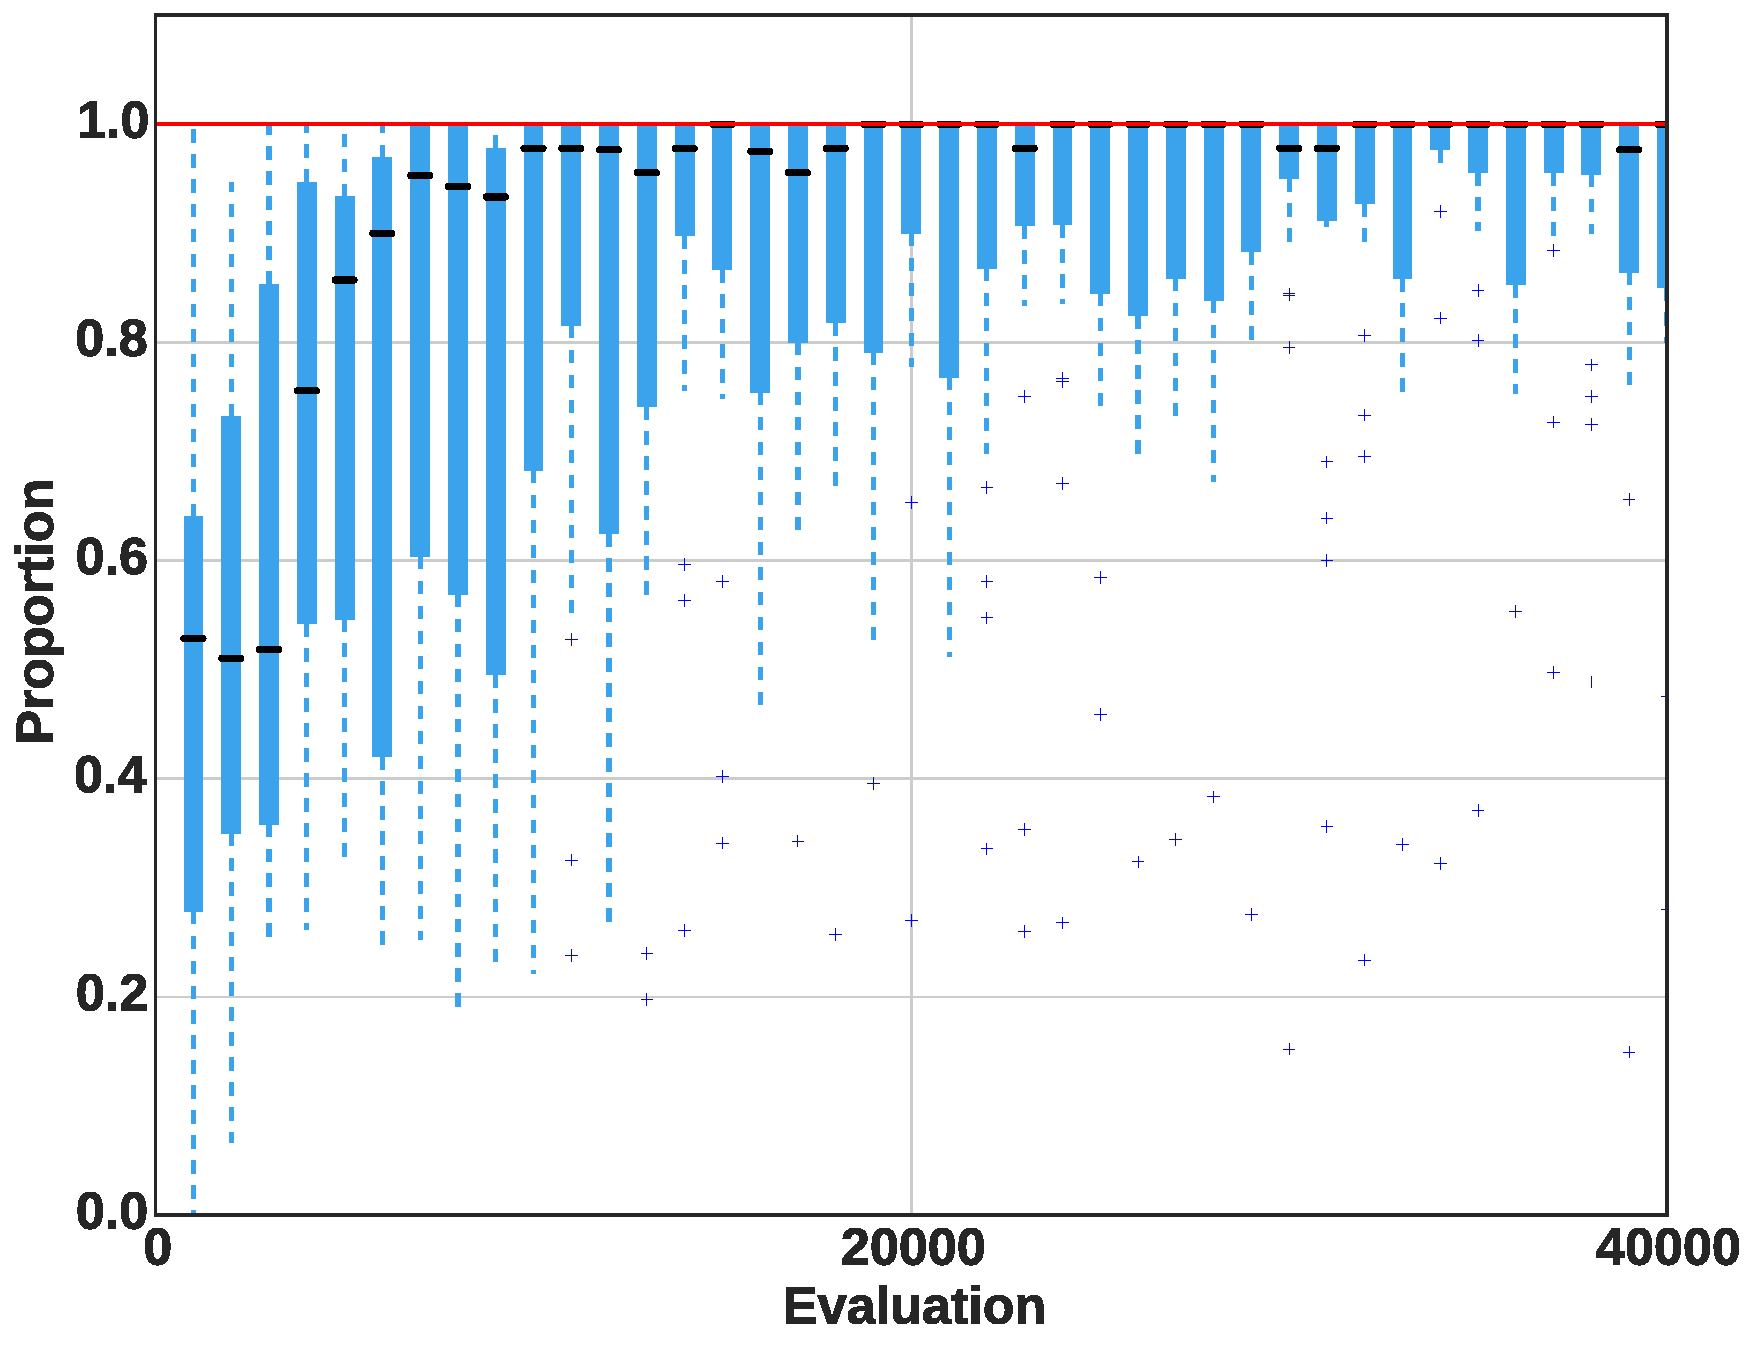
\includegraphics[scale=0.19]{fig/ArticleRob1/proportionLeadershipClonal.pdf}}
      \end{subfigure}
      \begin{subfigure}[]
        {\label{fig:leadershipCoevo} 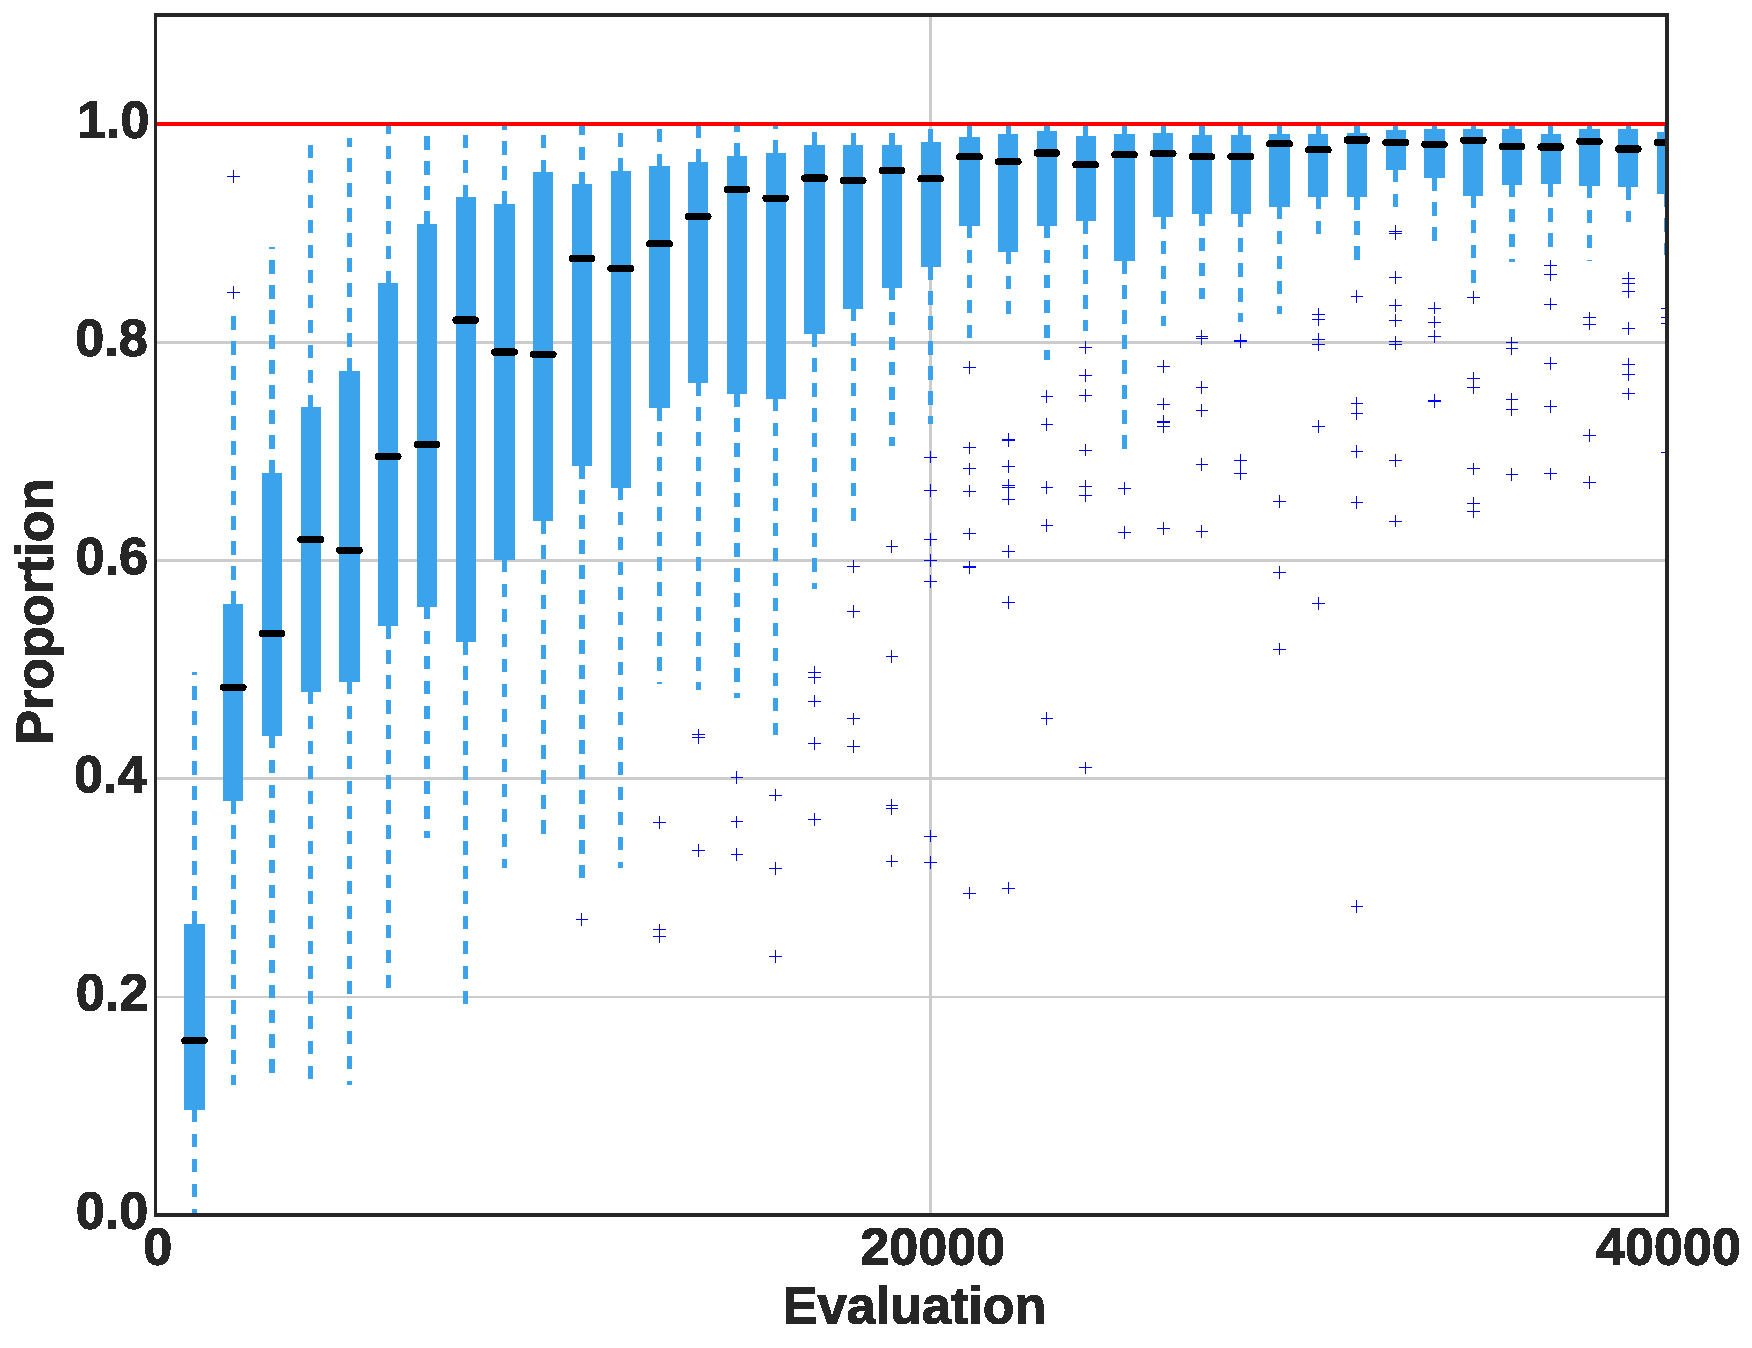
\includegraphics[scale=0.19]{fig/ArticleRob1/proportionLeadershipCoevo.pdf}}
      \end{subfigure}
      \caption{Boxplots of the proportion of leadership over time for the best individuals in each runs where the proportion at the last evaluation was greater than 0.75 in the {\em (a)}~control, {\em (b)}~clonal or {\em (c)}~coevolution setup. This value represents the proportion of waypoints crossed by both individuals for which the leader arrived first.}
      \label{fig:WaypointsLeadership}
  \end{figure}

  In the coevolution setup, nearly all runs (59/60) evolved a leader/follower strategy. Interestingly, although fitness scores in the clonal and control setups are significantly different, this behavior evolved in roughly one third of the runs for both setups. To explain the difference in fitness scores, we must take into account the quality of the leader/follower strategy in each setup. We measure the proportion of leadership in each interaction, which is computed as the proportion of waypoints crossed by both individuals for which the leader arrived first. Figure~\ref{fig:WaypointsLeadership} displays the boxplots of the proportion of leadership for the best individuals in each setup and only for the simulations where a successful leader/follower strategy evolved (a minimal threshold of 0.75 is chosen to consider only the best performing runs). We show that the proportion of leadership is greater in the clonal and coevolution setups than in the control one (Mann-Whitney, {\em p}-value $< 0.005$). These differences means that the individuals are more efficient in their leader/follower strategy in the clonal and coevolution settings than in the control one. This explains the differences in fitness scores observed in Figure~\ref{fig:WaypointsFitness}.

  Interestingly, whereas in the foraging task no leader/follower strategy could evolve in the control and clonal setups, this strategy did evolve in one third of the simulations for this task. This could mean that these individuals use information in the environment to adopt one role or the other. Indeed, we observe that this is achieved by exploiting the differences in the initial starting positions, with one individual on the left and the other on the right. They both turn to the same direction (left or right, depending on the runs) at the beginning of the simulation which results in one individual (the leader) turning its back to the other, while the second individual (the follower) looking at its partner. 


  \subsubsection{Recycling Cooperative Behaviors in the Foraging Task}

  Coming back to the initial foraging task, we perform the exact same experiment described at the beginning of this paper, with one notable exception: the initial population is initialized with genomes evolved for solving the waypoint task. This implies that coordination is possible starting from the very first generation of each setup. Given that we have already shown that such coordination is a desirable feature, the question is: will it be possible to retain cooperative behaviors in order to solve the foraging task?

  \begin{table}[hbtp]
    \center{
      \begin{tabular}{lcccc}
        \hline
        \multirow{2}{*}{\textbf{Setting}} & \multicolumn{2}{c}{\textbf{\# Coop.}} & \multirow{2}{*}{\textbf{\# Solitary}} & \multirow{2}{*}{\textbf{Total}}\\ 
        \cline{2-3}
         & \textbf{\# Lead.} & \textbf{\# Turn.} & & \\ 
        \hline
        \textit{Control} & 0 & 20 & 40 & \textbf{60}\\
        \textit{Clonal} & 0 & 24 & 36 & \textbf{60}\\
        \textit{Coevolution} & 28 & 0 & 32 & \textbf{60}\\
        \hline
      \end{tabular}
    }
    \caption{Proportion of the 60 independent simulations where the best individual evolved a cooperative strategy (collecting purple targets) or a solitary strategy (collecting green targets) for each setup in the foraging task when individuals are previously evolved in the waypoints task. In addition, the repartition of the different strategies is indicated when cooperation evolved: \emph{Leader/Follower} (Lead.) or \emph{Turning} (Turn.).}
    \label{tab:RecyclingCoopBehaviors}
  \end{table}

  Table~\ref{tab:RecyclingCoopBehaviors} gives the results in terms of evolved behaviors from the $60$ independent runs for each setup. 
  The coevolution setup evolves cooperation slightly more often (28/60) than both the control (20/60) and the clonal (24/60) setups. 
  A first remark is that the number of occurences of cooperation for the coevolution and control setups have actually doubled compared to previous results without incremental evolution (see Table~\ref{tab:ForagingCoop}). This is not the case for the clonal setup, which does not appear to benefit from incremental evolution. 

  A second remark is that cooperation in the coevolution setup systematically corresponds to a leader/follower strategy, which is \textit{never} the case with the two other setups. This has a significant, though expected, impact on fitness scores, as shown in Figure~\ref{fig:RecyclingFitness}. Cooperation evolved with the coevolution setup leads to significantly greater fitness scores (Mann-Whitney, {\em p}-value $<0.001$). 

  Results from this experiment make it possible to revise our initial statement. Using pre-trained individuals strongly benefits the coevolution setup in terms of evolvability. But this is not the case with the clonal setup, for which using pre-trained individuals improves neither evolvability nor efficiency. Therefore, we may face a tradeoff which does not concern evolvability and efficiency, but one that implies computational cost: the coevolution setup outperforms the clonal setup on both evolvability and efficiency \textit{at the cost of additional computational effort}.

  The control and clonal setups completely failed to maintain a leader/follower strategy, even though such strategy originally evolved. An explanation is provided by considering the difference between the waypoints task, where leader/follower evolved, and the current foraging task. In the waypoints task, symmetry breaking could be achieved at the beginning of the evaluation (as explained earlier), and could be retained afterwards as the follower was always behind the leader. However, the current foraging setup requires that the two robots display the same behavior to cooperatively collect a target (ie. both robots have to touch the target), which implies that leader/follower roles are lost, as they depend on the relative position of robots with one another. 


  \begin{figure}[hbtp]
    \begin{center}
      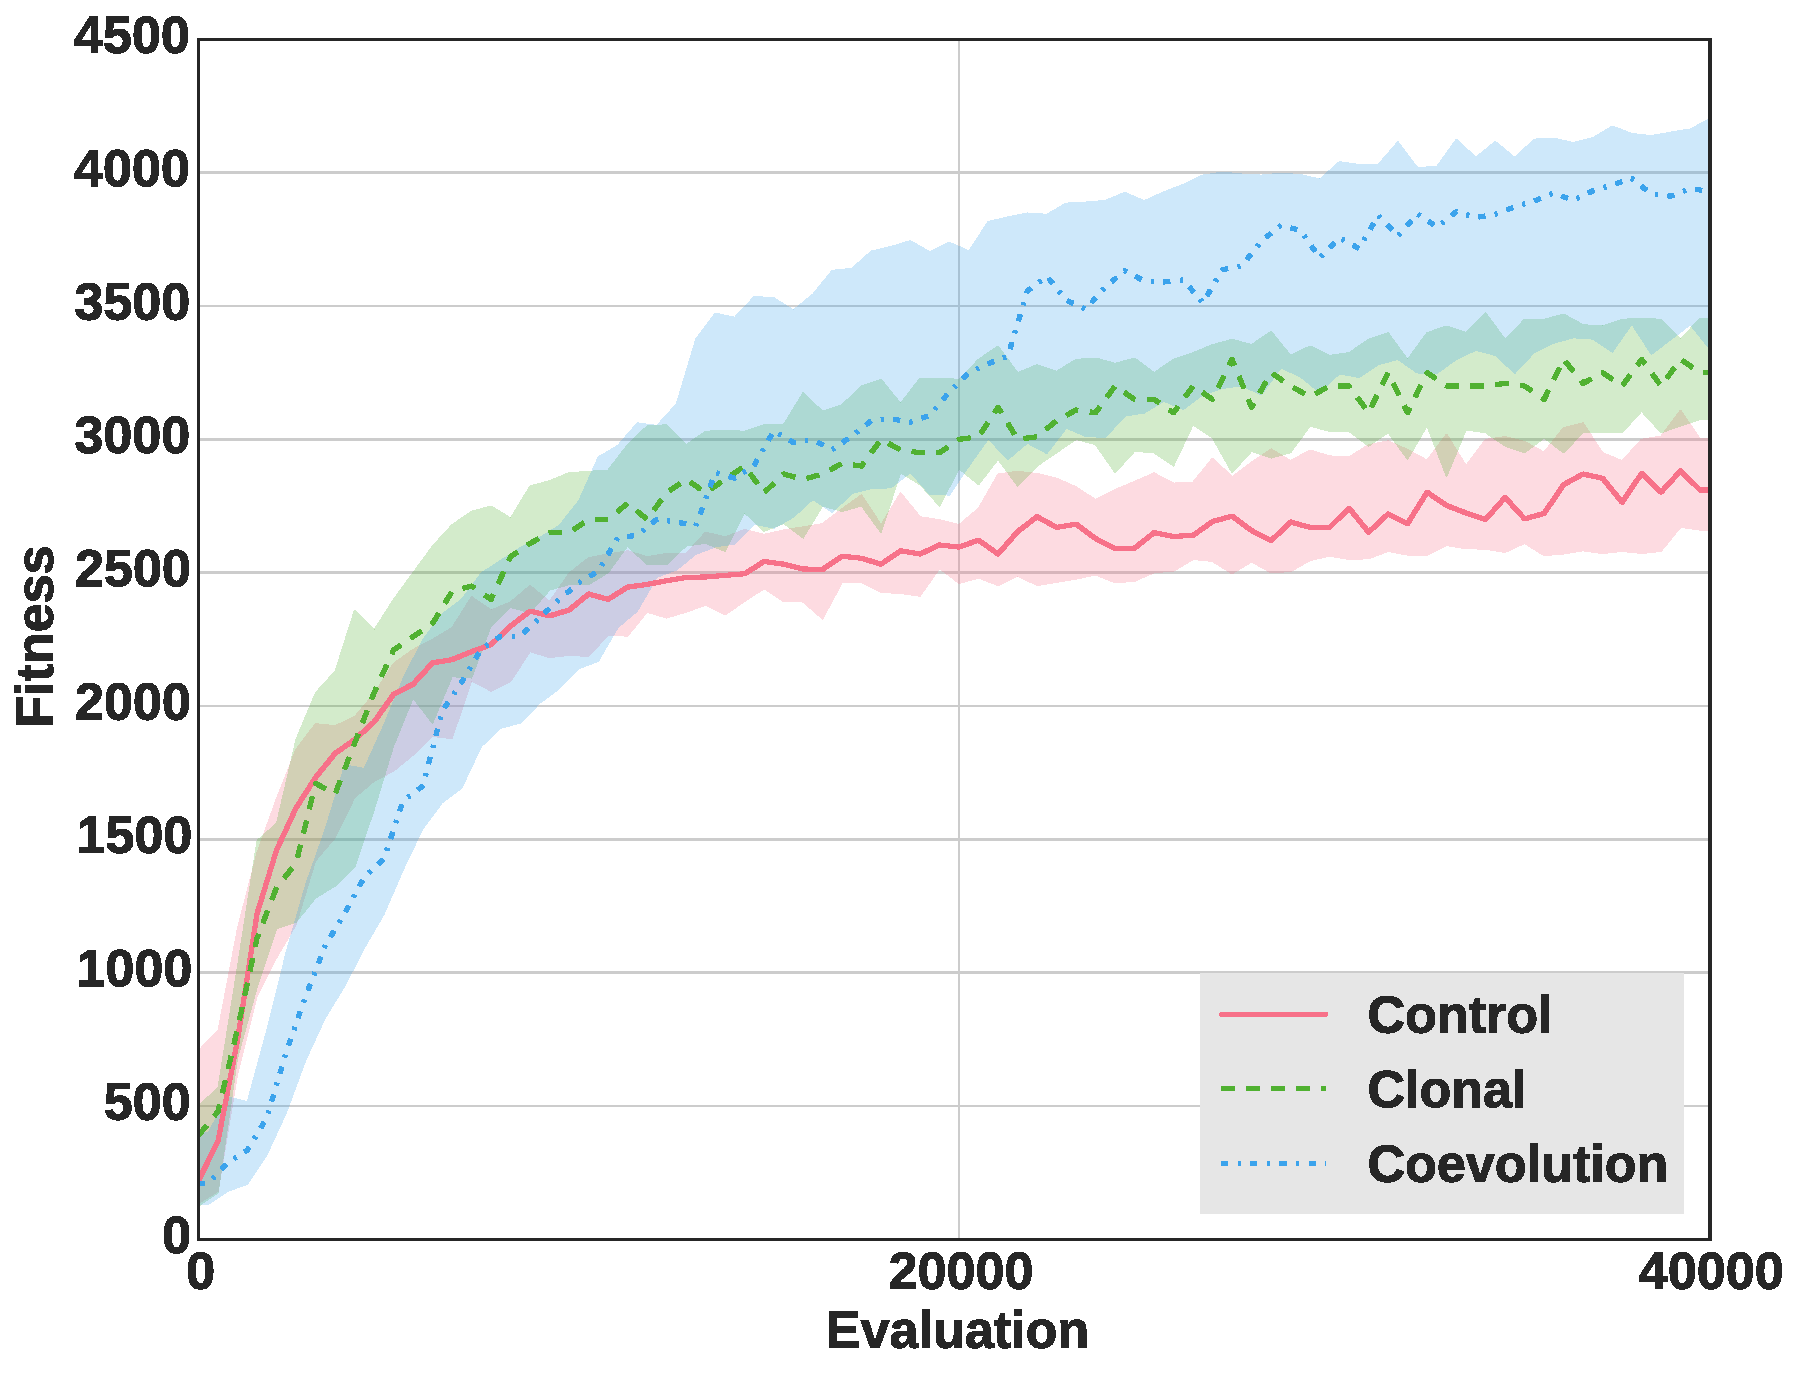
\includegraphics[scale = 0.3]{fig/ArticleRob1/fitnessRecyclingStags.pdf}
      \caption{Median fitness score of the best individuals in each of the runs where cooperation evolved for each setup over time. The fitness score of an individual is computed as the average reward the individual earned per trial by foraging targets. The colored areas around the medians represent the first and third quartiles.}
      \label{fig:RecyclingFitness}
      \end{center}
  \end{figure}

  \subsection{Discussion and Conclusion}

  In this paper, we considered several approaches for the evolution of cooperation in evolutionary robotics: a clonal approach, where all individuals in a group share the same genome, and a non-clonal approach, where individuals are independent from one another, but may share a common interest in cooperating. 

  We first showed that there exists a tradeoff between evolvability and efficiency. On the one hand, the clonal approach evolves cooperative behaviors on a more frequent basis than with the other approach. On the other hand, the non-clonal approach, which is implemented using a coevolution setup, results in more efficient behaviors in terms of pure performance whenever cooperation evolved. The non-clonal approach actually enables the evolution of asymmetric behaviors, such as a leader/follower strategy.

  We then used incremental evolution to evolve coordination behaviors using a simpler task in order to overcome this tradeoff and improve both evolvability and efficiency in each setup. We showed that while no improvement was observed in the clonal setup on either criteria, the outcome is very different for the coevolution setup: the probability of evolving cooperation actually increases, and the evolved cooperative solutions remain the most efficient.
 
  This work raises several questions. Firstly, heterogeneous behaviors were obtained with coevolution, a rather radical way to enable asymmetrical behaviors during cooperation. However, the waypoints task revealed that breaking symmetry can also be done with identical individuals using environmental feedback, even though such cooperation is difficult to obtain. As a consequence, we intend to investigate the evolution of cooperation with heterogeneous behavior without resorting to coevolution. In particular, we will study how more elaborated neural architectures (e.g. using plasticity) can switch to a particular persistant regime depending on environmental cues available at the beginning of the evaluation.

  Secondly, incremental evolution requires an added computational cost in order to increase evolvability in the non-clonal approach. However, it may be possible to avoid this extra cost by considering other evolutionary methods. In particular, we intend to explore how a multiobjective approach which considers both performance and \emph{diversity} could improve the optimization process~\cite{Lehman2008, Doncieux2014}. Though this approach looks promising, it is not clear yet how diversity should be implemented in the context of cooperative problem solving.


\section{Evolving Specialisation in a Population of Heterogeneous Robots: the Challenge of Bootstrapping and Maintaining Genotypic Polymorphism}
  \subsection{Introduction}
    Task specialisation is a defining characteristic in achieving efficient coordination and is thus considered to be crucial in the evolution of complex cooperative behaviours~\cite{Eors1995}. The problem of evolving cooperation has been largely studied in evolutionary robotics as it raises interesting persepectives for the design of collective robotics~\cite{Trianni2007, Hauert2014, Doncieux2015}. As a consequence, the manner in which robotic agents could evolve specialisation (or division of labour) for a cooperative task represents a compelling challenge in evolutionary robotics. As such, a large body of litterature has already been dedicated to this subject. However, most research focus on the particular case of homogeneous groups of individuals~\cite{Waibel2009} as is classic in evolutionary robotics. This means that the individuals are forced to rely on phenotypical plasticity~\cite{Waibel2006, Ferrante2015, Eskridge2015} and/or environmental cues~\cite{Waibel2006, Goldsby2010} in order to achieve specialisation. In comparison, the evolution of specialisation in a population of unrelated individuals has been mostly ignored.

    Yet achieving division of labour under such conditions raises an interesting problem: because individuals cannot dynamically specialise during evaluation, the division needs to occur at the genotypic level. Thus it poses the problem of both \emph{evolving} and \emph{maintaining} genotypic polymorphism in a single population. Here we investigate the conditions under which specialised behaviours for a cooperative task can evolve in a single population of heterogeneous individuals. In particular, we are interested in the influence of the selection process in achieving division of labour. 

    We design a 2-robots cooperative foraging task where both a solitary and a cooperative strategies can evolve but where cooperation is highly rewarded. The genotype of each robotic agent is separately chosen in the population and the individuals therefore form an heterogeneous group. This task is greatly favored by the evolution of efficient coordination strategies. In particular, our previous work on a similar task~\cite{Bernard2015} showed that two types of cooperative strategy could evolve: one where both individuals adopt homogeneous behaviours (generalists) and the other one where they adopt a leader/follower strategy (specialists). As the latter is the more efficient one we study the conditions for its emergence. The evolutionary dynamics of two popular selection methods are studied: (1) an elitist \((\mu + \lambda)\) selection scheme and (2) a fitness-proportionate selection scheme. Fitness-proportionate in particular is interesting with regards to genotypic polymorphism as it is known to allow the evolution of frequency-dependent selection~\cite{Altenberg1991}.

    In the next Section, we introduce the experimental setup. Then we present the two types of successful cooperative strategies that may evolve. Next, we investigate whether any of the selection methods could evolve heterogeneous behaviours. In particular, we study for both schemes the evolutionary outcomes depending on whether the population is initially constituted of random individuals or seeded with pre-evolved efficient specialists. Then we present the results of computational analyses in order to reveal and understand more deeply the mechanisms at play. In a final experiment, we reveal two key properties required for the evolution of heterogeneous behaviours, and discuss the implications of our work.




  \subsection{Methods}
  \label{sec:methods}
    We evaluate two robotic agents in a $800$ by $800$ units square arena devoid of any obstacle except for the foraging targets. At the beginning of a simulation, $18$ targets are randomly positioned in the environment. While the agents may move freely in the arena, the targets' positions are fixed. For a target to be collected, any agent needs to stay in contact with it for a specified amount of time ($800$ simulation steps). The target is removed after this duration and put back at another random position so that the number of targets is kept the same throughout a simulation. We consider that cooperative foraging happens if both individuals are in contact of the target when it is removed. When an agent collects a target, it is rewarded 50 if this target has been foraged in a solitary manner or 250 if both agents have cooperated to collect it.

    Each agent is circular-shaped with a diameter of $20$ units and possesses a collection of different sensory inputs. The first type of inputs is a $90$ degrees front camera and is composed of $12$ rays, each one indicating the type and distance to the nearest object (either another agent or a target). The other type of inputs are $12$ proximity sensors evenly distributed around the agent's body. With a range of twice the agent's diameter, each proximity sensor outputs the proximity of the nearest obstacle in its range.

    Both agents begin the simulation next to each other at the same end of the arena and can move according to the outputs of their neural network. This neural network is a fully connected multi-layer perceptron with one hidden layer. The inputs of the neural network are comprised of all the sensory information of the agent, i.e. $36$ input neurons for the camera ($3$ inputs for each ray) and $12$ for the proximity sensors. A final input neuron whose value is always $1$ is used as a bias neuron. This amounts the total number of input neurons to $49$. The hidden layer is constituted of $8$ neurons while the $2$ neurons of the output layer return the speed of the agent's wheels. A sigmoid is used as the activation function of each neuron. Finally, the topology of the network is kept constant during the experiments.

    The population of individuals is evolved thanks to a classical evolutionary algorithm. The genotype of each individual is constituted of a collection of the $410$ real-valued connection weights of the neural network. At each generation of the algorithm, every individual is evaluated by being paired $5$ times with other individuals randomly chosen in the population (i.e. $5$ 1-to-1 pairing). Each pair interacts in the setting presented before during $20000$ simulation steps which we call a \emph{trial}. We perform $5$ trials for each pair of individuals in order to decrease the impact of the targets' random positions on the individuals' performance. The fitness score (\(F\)) of an individual is computed as the average reward per trial:

    \[
    F = \frac{1}{N*M} \sum_{i=1}^{N} \sum_{j=1}^{M} f_{ij}
    \]

    with \(N\) the number of partners the individual is paired with ($5$), \(M\) the number of trials with each partner ($5$) and \(f_{ij}\) the sum of rewards obtained at trial \(j\) with partner \(i\).

    The population for the next generation is created according to two different selection schemes:

    \begin{itemize}
      \item{\textbf{\((\mu + \lambda)\) elitist selection:} the population of the next generation is constituted of the $\mu$ best individuals from this generation and $\lambda$ offsprings built from the best individuals.}
      \item{\textbf{Fitness-proportionate:} offsprings are built by sampling individuals from the current generation to constitute the population of the next generation. The probability to sample a particular parent is proportional to this parent's fitness score.}
    \end{itemize}

    Regardless of the selection method used, every offspring is a mutated clone of its parent and no recombination is used in our algorithm. The probability for each gene to mutate is \(5 \times 10^{-3}\) and mutations are sampled according to a gaussian operator with a standard deviation of \(2 \times 10^{-2}\). Finally, experiments were conducted with the robotic 2D simulator of SFERESv2~\cite{Mouret2010}, a framework for evolutionary computation. Source code for the experiments is available for download at http://pages.isir.upmc.fr/\textasciitilde bredeche/Experiments/ALIFE2016-specialisation.tgz
    

  \subsection{Behaviours of Specialists in a Cooperative Foraging Task}
  \label{sec:efficiency}
    We showed in a previous article~\cite{Bernard2015} that two cooperative strategies could evolve in this particular task: \emph{turning} (between two \emph{turners}) and \emph{leader/follower} (between a \emph{leader} and a \emph{follower}). Both of these strategies achieve cooperative foraging but with varied efficiency.

    \begin{figure}[hbtp]
      \centering
        \begin{subfigure}[]
          {\label{fig:behaviorTurning} 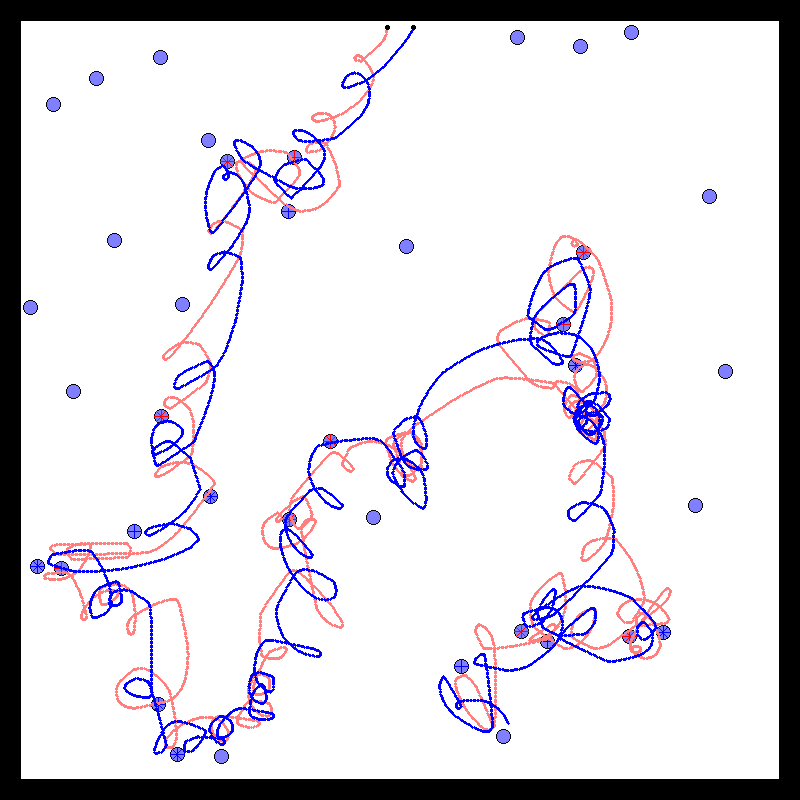
\includegraphics[scale=0.14]{fig/ArticleRob2/behaviorTurning.png}}
        \end{subfigure}~
        \begin{subfigure}[]
          {\label{fig:behaviorLeadership} 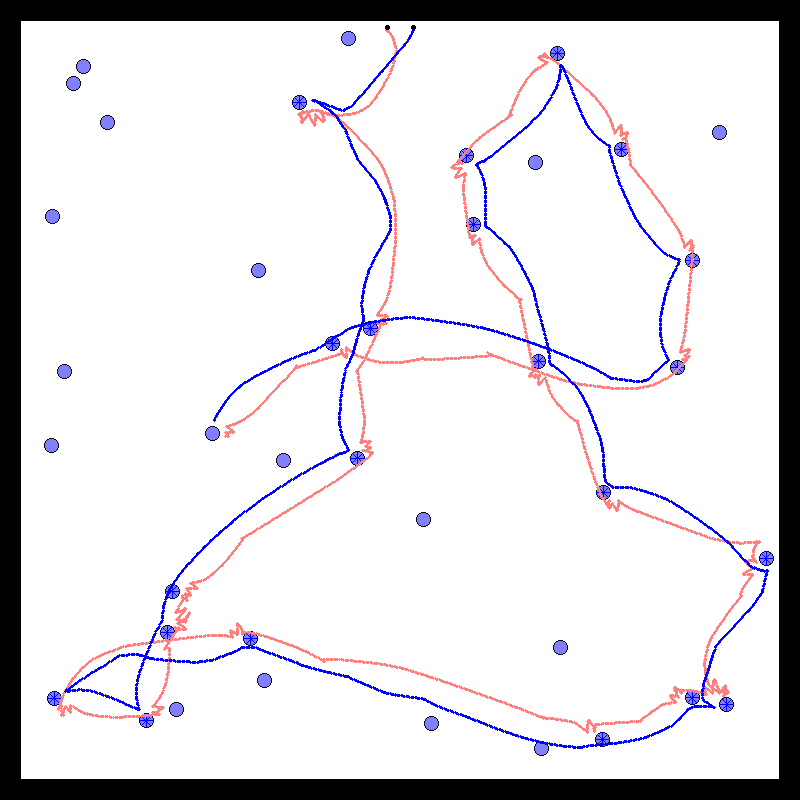
\includegraphics[scale=0.14]{fig/ArticleRob2/behaviorLeadership.png}}
        \end{subfigure}
        \caption{\textbf{Snapshots of the simulation after an entire trial in the foraging task.} The path of each robotic agent from their initial positions (black dots) is represented in red and blue. The blue discs represent the 18 targets in the environment. When a target is foraged by the two agents, a red cross (resp. blue) is drawn on the target if the red agent (resp. blue) arrived on it first. Each snapshot corresponds to a trial where agents adopted a different behavior: {\em (a)}~turning or {\em (b)}~leader/follower.}
        \label{fig:behaviorTraces}
    \end{figure}

    In the turning strategy, both individuals turn around one another so that they can keep the other individual in their line of sight and stay close to it (see Figure \ref{fig:behaviorTurning}). At the same time, the two individuals try to get closer to a target. This way, as soon as one of the two individuals is in contact with a target, the other individual can join it so the target may be collected cooperatively. Consequently, both individuals adopt a similar behaviour in this strategy and can be described as generalists.

    In the leader/follower strategy, the individuals specialise in two roles: a \emph{leader} and a \emph{follower}. The \emph{leader} always gets on the target first and checks rarely for its partner. In comparison, the \emph{follower} tries to keep its \emph{leader} in view during the entirety of the simulation so that it can get on the same target (see Figure \ref{fig:behaviorLeadership}). Consequently, we observe the expression of two clearly heterogeneous behaviours which implies that both individuals are specialists.

    \begin{figure}[hbtp]
      \centering
        \begin{subfigure}[]
          {\label{fig:Efficiency} 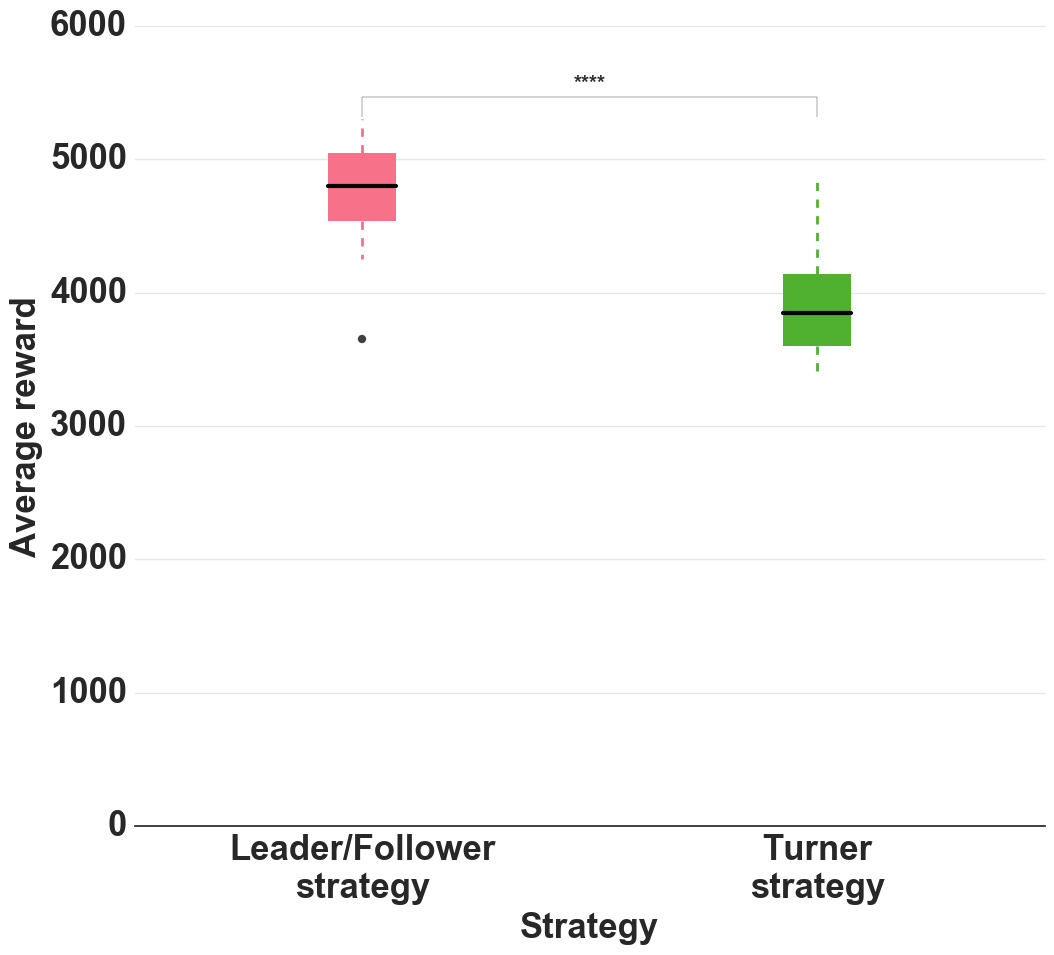
\includegraphics[scale=0.25]{fig/ArticleRob2/boxplotFitness.png}}
        \end{subfigure}~
        \begin{subfigure}[]
          {\label{fig:Leadership} 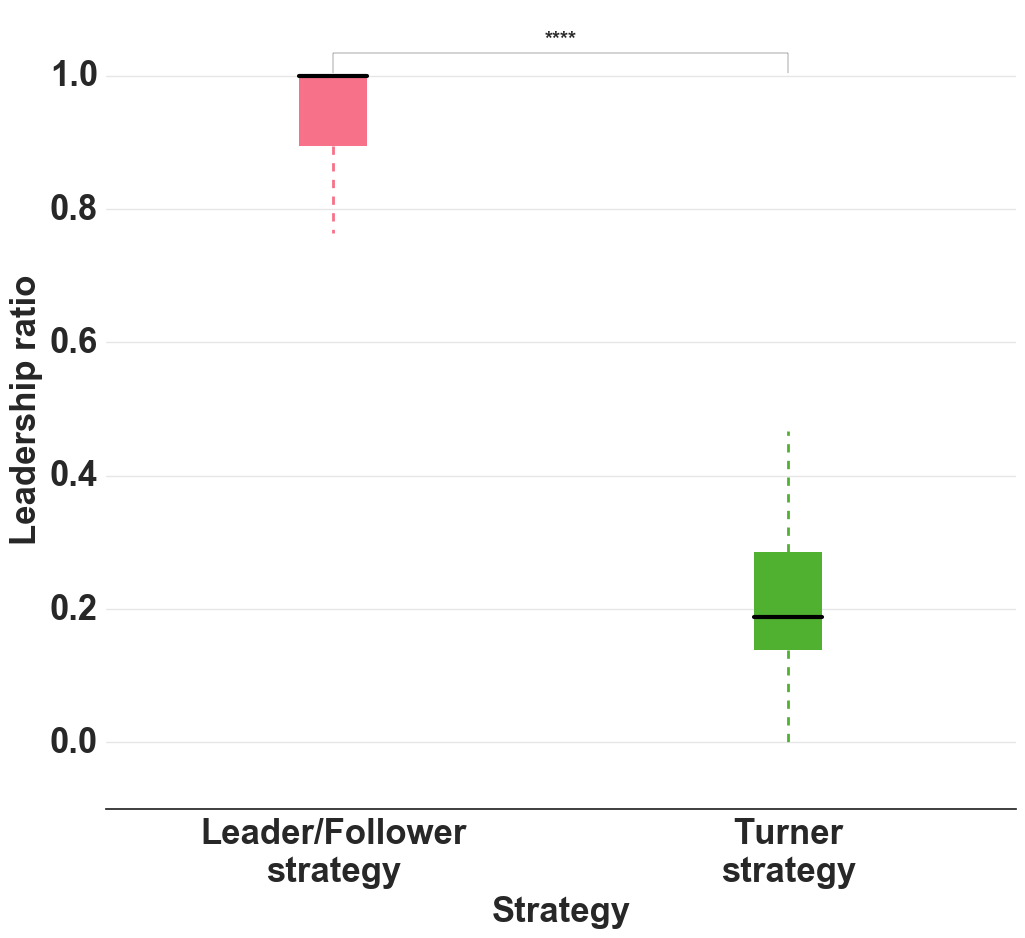
\includegraphics[scale=0.25]{fig/ArticleRob2/boxplotLeadership.png}}
        \end{subfigure}
        \caption{\textbf{Average reward and leadership proportion with a leader/follower or turning strategy} Boxplots of {\em (a)}~the average reward and {\em (b)}~the leadership proportion over $20$ independent trials for the leader/follower and turning strategies. The leadership ratio of an individual represents the propensity for one individual among the pair to arrive first more often than its partner on a target collected in a cooperative fashion. The position of each target at the beginning of each trial was randomized.}
        \label{fig:EfficiencyAndLeadership}
    \end{figure}

    Figure~\ref{fig:Efficiency} shows the efficiency of each strategy, defined as the average reward obtained of the two individuals during a simulation over $20$ independent trials (with randomized targets' positions for each trial). We can see that, as expected, the leader/follower strategy achieves a significantly higher efficiency (Mann-Whitney U-test on the average reward over $20$ trials, {\em p}-value $< 0.0001$). This difference in efficiency is directly correlated to a highly significant difference in the proportion of leadership as shown in Figure~\ref{fig:Leadership} (Mann-Whitney U-test on the leadership proportion over $20$ trials, {\em p}-value $< 0.0001$). We compute this proportion by looking at the propensity for one of the two individuals to arrive first more often on a target foraged cooperatively.



  \subsection{Evolving Heterogeneous Behaviours with an Elitist Selection}
  \label{sec:elitistEvolution}
    \subsubsection{Bootstrapping leader/follower strategies}
      In this first experiment, we are interested in the emergence of a leader/follower strategy when starting with a population of random individuals under an \((\mu + \lambda)\) elitist selection. In order to investigate the influence of population size, we tested three different sizes \(N\): $20$, $40$ and $100$. For each population size, we conducted $11$ independent runs, each one lasting $90000$ evaluations. For each population size \(N\), we defined \(\mu\) (i.e. the number of parents) and \(\lambda\) (i.e. the number of offsprings) as follows:
        \[
          \mu = \frac{N}{2}, 
          \lambda = \frac{N}{2}
        \]

      For example, when population size was $100$, $50$ individuals were kept from the previous generation and used to create $50$ mutated offsprings.

      \begin{table}[hbtp]
        \center{
          \begin{tabular}{lcccc}
            \hline
            \textbf{Pop.} & \textbf{\# L/F} & \textbf{\# Turning} & \textbf{\# NC} & \textbf{Total}\\ 
            \textbf{size} & \textbf{Strat.} & \textbf{Strat.} & \textbf{Strat.} & \\ 
            \hline
            \textit{20} & 0 & 11 & 0 & \textbf{11}\\
            \textit{40} & 0 & 11 & 0 & \textbf{11}\\
            \textit{100} & 1 & 10 & 0 & \textbf{11}\\
            \hline
          \end{tabular}
        }
        \caption{\textbf{Strategies evolved by the best individuals under elitist selection with an initially random population.} Repartition of the different strategies adopted by the best individuals at the last evaluation in each of the replicates for different population sizes \(N\). We indicate in each cell the number of simulations where a particular strategy evolved. Populations were evolved under an \((\mu + \lambda)\) elitist selection, with \(\mu = \frac{N}{2}\) and \(\lambda = \frac{N}{2}\). Individuals' genotype values were intially random. In the table "L/F" stands for leader/follower and "NC" for "Non-Cooperative".}
        \label{tab:elitistScratchStrategies}
      \end{table}

      Table~\ref{tab:elitistScratchStrategies} shows the repartition of the best individuals' strategies at the last generation of evolution for each population size. We consider a behaviour to be cooperative when more than 50\% of the total number of targets collected are foraged cooperatively. First we observe that in every replicates, individuals always end up evolving a cooperative strategy. We also see that evolving a leader/follower strategy is difficult as specialists evolve in only $1$ run (out of $33$) and when the population size is $100$. These results suggest that it is nearly impossible to evolve such heterogeneous behaviours with this setting.

      However, when looking at the whole evolutionary history we can reveal additional information about the evolution of specialists. We show in Figure~\ref{fig:leadershipTime} the proportion of evolutionary time when the best individual of each run adopted a leader/follower strategy. This value is computed as the ratio of the number of generations when the leadership ratio was high enough (threshold value of $0.6$) out of the total number of generations. We observe that even if the best individuals end up adopting a generalist strategy, this was not the case during the entirety of the evolution. In particular, there is a significant increase (Mann-Whitney, {\em p}-value $< 0.05$) in the number of generations where the best individual showed a leader/follower strategy when population size was $100$ compared to a population size of $20$. Therefore this implies that it is possible to evolve specialists but their stability in the population over time is nearly impossible to achieve.

      \begin{figure}[hbtp]
        \centering
          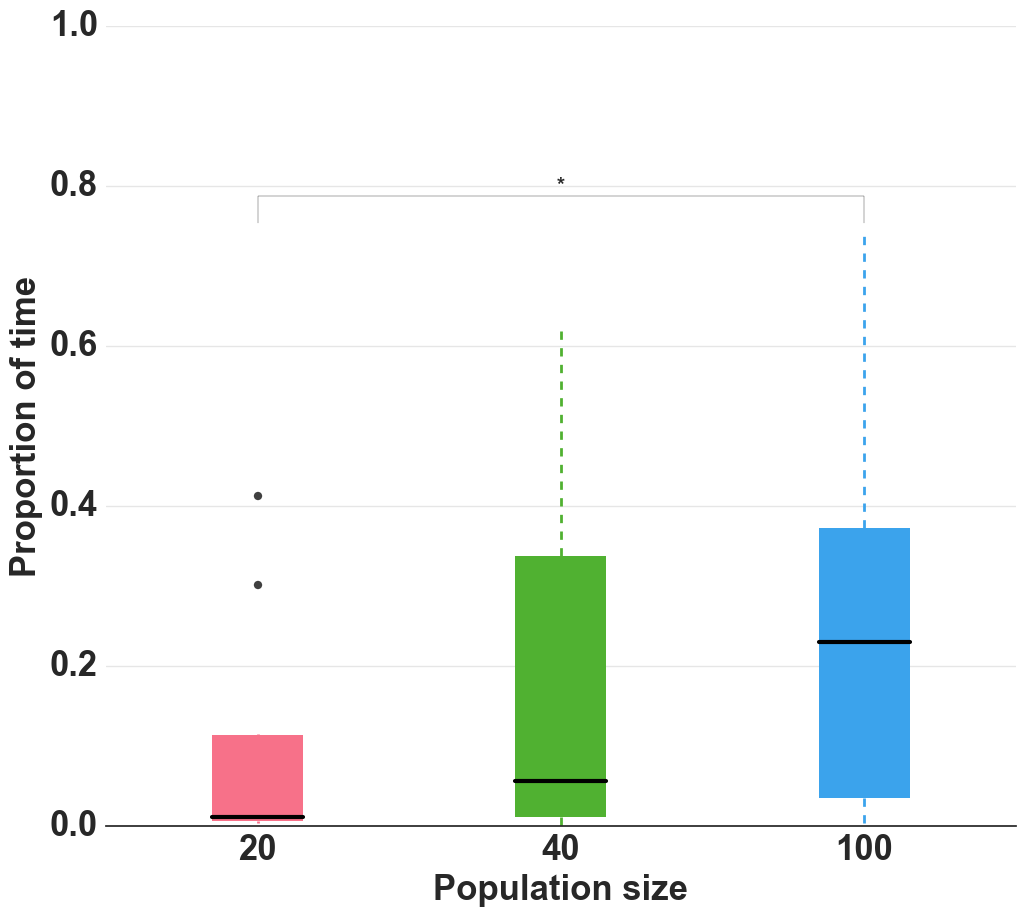
\includegraphics[scale=0.25]{fig/ArticleRob2/boxplotLeadershipTime.png}
          \caption{\textbf{Proportion of time with a leader/follower strategy.} Boxplots of the number of generations when the best individual in each replicate adopted a leader/follower strategy out of the total number of generations. We consider that the best individual adopted a leader/follower strategy when its leadership ratio was over a threshold value of $0.6$.}
        \label{fig:leadershipTime}
      \end{figure}


    \subsubsection{Maintaining heterogeneity in a population seeded with specialists}
      In order to investigate the lack of stability of genotypic polymorphism under elitist selection, we design another experiment. We separately evolve a population of non-cooperators, which we call \emph{solo} individuals (i.e. \emph{leaders}), and efficient \emph{follower} beforehand. We then replace the worst individuals w.r.t. fitness score in the population of solo individuals by a certain amount of \emph{followers}. Our goal is to study if artificially constructing such population could result in the invasion and fixation of a stable leader/follower strategy.

      The number of \emph{followers} initially inserted in the population was varied according to two different settings: (1) we add only one \emph{follower} or (2) we add an amount of \emph{followers} equal to half of the population. Experiments were replicated $11$ times during $90000$ evaluations with population size of $40$ and $100$.

      \begin{table}[hbtp]
        \center{
          \begin{tabular}{lrcccc}
            \hline
            \textbf{Pop.} & \textbf{Followers} & \textbf{\# L/F} & \textbf{\# Turning} & \textbf{\# NC} & \textbf{Total}\\ 
            \textbf{size} & \textbf{added} & \textbf{Strat.} & \textbf{Strat.} & \textbf{Strat.} & \\ 
            \hline
            \textit{40} & \textit{1} & 0 & 11 & 0 & \textbf{11}\\
            \textit{40} & \textit{20} & 0 & 11 & 0 & \textbf{11}\\
            \textit{100} & \textit{1} & 1 & 10 & 0 & \textbf{11}\\
            \textit{100} & \textit{50} & 2 & 9 & 0 & \textbf{11}\\
            \hline
          \end{tabular}
        }
        \caption{\textbf{Strategies evolved by the best individuals with elitist selection when adding \emph{followers}.} Repartition of the different strategies adopted by the best individuals at last evaluation in each of the replicates for different population sizes \(N\). We indicate in each cell the number of simulations where a particular strategy evolved. Populations were evolved under a \((\mu + \lambda)\) elitist selection, with \(\mu = \frac{N}{2}\) and \(\lambda = \frac{N}{2}\). The population was initially seeded with a population of \emph{solo} individuals in which we added a specific amount of \emph{followers}. In the table "L/F" stands for leader/follower and "NC" for "Non-Cooperative".}
        \label{tab:elitistInvasionStrategies}
      \end{table}


      We show (Table~\ref{tab:elitistInvasionStrategies}) no significant differences in comparison with a population constituted of initially random individuals w.r.t. the number of simulations where a leader/follower strategy evolved. These results suggest that even when purposely adding specialists, their stability in the population is still very hard to achieve. This implies that whether the behaviours are evolved from random genotypes or bootstrapped with efficient individuals is not as important as maintaining heterogeneity in the population. In particular, in only one replicate among the $3$ runs where a leader/strategy was eventually adopted (out of $44$) did the specialists initially added were maintained. In the $2$ other runs we observe multiple emergences and disappearances of specialists throughout evolution. 

      % TODO: Mentionner que néanmoins le leader/follower est globalement plus stable comparé du from scratch ?
      % However, it is interesting to note that the addition of efficient followers lead to more stable heterogeneity than when starting from scratch [TODO: GRAPH LEADERSHIP TIME].


  \subsection{Evolution Under a Fitness-Proportionate Selection}
  \label{sec:fitpropEvolution}
    In this next experiment we want to investigate the evolution of heterogeneous behaviours when using a fitness-proportionate selection. As fitness-proportionate is known to allow frequency-dependent selection, we hypothesize that it may facilitate the evolution of specialists.

    \subsubsection{Bootstrapping leader/follower strategies}
      Similarly to the elitist selection, we replicated our experiments in $11$ independent runs during $90000$ evaluations. Likewise, population sizes were $20$, $40$ and $100$. 
      
      \begin{table}[hbtp]
        \center{
          \begin{tabular}{lcccc}
            \hline
            \textbf{Pop.} & \textbf{\# L/F} & \textbf{\# Turning} & \textbf{\# NC} & \textbf{Total}\\ 
            \textbf{size} & \textbf{Strat.} & \textbf{Strat.} & \textbf{Strat.} & \\ 
            \hline
            \textit{20} & 0 & 1 & 10 & \textbf{11}\\
            \textit{40} & 0 & 1 & 10 & \textbf{11}\\
            \textit{100} & 1 & 2 & 8 & \textbf{11}\\
            \hline
          \end{tabular}
        }
        \caption{\textbf{Strategies evolved by the best individuals under fitness-proportionate selection with an initially random population.} Repartition of the different strategies adopted by the best individuals at the last evaluation in each of the replicates for different population sizes. We indicate in each cell the number of simulations where a particular strategy evolved. Populations were evolved under a fitness-proportionate selection. Individuals' genotype values were initially random. In the table "L/F" stands for leader/follower and "NC" for "Non-Cooperative".}
        \label{tab:fitpropScratchStrategies}
      \end{table}

      We show in Table~\ref{tab:fitpropScratchStrategies} that results are highly different when using such selection scheme. In particular, the fitness-proportionate selection performed poorly w.r.t. evolving cooperative strategies. For each population size, no cooperative strategy evolved at all in the vast majority of replicates. However in one particular run we do observe the emergence and fixation of specialists. This would suggest that fitness-proportionate may perform equally as an elitist selection w.r.t. the evolution of heterogeneous behaviours. 

      Yet a closer look at the dynamics of evolution under a fitness-proportionate selection yields interesting results. In particular, there is not much variation in the strategy adopted by the best individuals throughout evolution. This is consistent with the fact that the bootstrap of a cooperative strategy was not observed in most of the replicates: fitness-proportionate is not efficient in evolving any cooperative behaviour. In consequence, there is not much variation in the proportion of individuals adopting a leader/follower strategy during evolution. As a matter of fact, we observe that in the only replicate where there was genotypic polymorphism at the end of the simulation, specialists were already present at the random initialisation of the population and did not evolve through mutation. This is very different with the elitist selection where we observe multiple emergences of specialists (even briefly) during evolution in many different runs.

    \subsubsection{Maintaining heterogeneity in a population seeded with specialists}
      \begin{table}[hbtp]
        \center{
          \begin{tabular}{lrcccc}
            \hline
            \textbf{Pop.} & \textbf{Followers} & \textbf{\# L/F} & \textbf{\# Turning} & \textbf{\# NC} & \textbf{Total}\\ 
            \textbf{size} & \textbf{added} & \textbf{Strat.} & \textbf{Strat.} & \textbf{Strat.} & \\ 
            \hline
            \textit{40} & \textit{1} & 7 & 0 & 4 & \textbf{11}\\
            \textit{40} & \textit{20} & 8 & 0 & 3 & \textbf{11}\\
            \textit{100} & \textit{1} & 10 & 0 & 1 & \textbf{11}\\
            \textit{100} & \textit{50} & 10 & 0 & 1 & \textbf{11}\\
            \hline
          \end{tabular}
        }
        \caption{\textbf{Strategies evolved by the best individuals with fitness-proportionate selection when adding \emph{followers}.} Repartition of the different strategies adopted by the best individuals at the last evaluation in each of the replicates for different population sizes \(N\). We indicate in each cell the number of simulations where a particular strategy evolved. Populations were evolved under a fitness-proportionate selection. The population was initially seeded with a population of \emph{solo} individuals in which we added a specific amount of \emph{followers}. In the table "L/F" stands for leader/follower and "NC" for "Non-Cooperative".}
        \label{tab:fitpropInvasionStrategies}
      \end{table}

      As expected from previous results, fitness-proportionate performs well in terms of stability of heterogeneous behaviours. We show in Table~\ref{tab:fitpropInvasionStrategies} that in the majority of replicates the best individuals adopt a leader/follower strategy at the end of the simulations. This is particularly true when population size is high enough ($100$). A major difference with the elitist selection is that in all replicates where a leader/follower strategy was observed at the end of the run, the specialists were maintained from the start throughout evolutionary time. These results suggest that, although not efficient at bootstrapping cooperative behaviours, fitness-proportionate performs well w.r.t. the stability of genotypic heterogeneity.


    \subsection{Computational Analyses of Population Dynamics}
      In this Section, we aim at understanding more deeply the dynamics at play that allow the invasion of suboptimal generalists even when efficient specialists are present. To that end we run computational analyses based on the expected fitness of each of the three phenotypes. Table~\ref{tab:payoffMatrix} shows the average payoff of pair-wise simulations between each type of phenotypes. We consider the payoffs for both phenotypes in each pair to be identical as no significant differences were observed between their payoffs.

      \begin{table}[hbtp]
        \center{
          \begin{tabular}{cccc}
            \hline
            \textbf{Phenotype} & \textit{Solo} & \textit{Follower} & \textit{Turner} \\
            \hline
            \textit{Solo} & 1265 & 5000 & 3480 \\
            \textit{Follower} & 5000 & 100 & 2750 \\
            \textit{Turner} & 3480 & 2750 & 2755 \\
            \hline
          \end{tabular}
        }
        \caption{\textbf{Payoff matrix for pair-wise simulations of each phenotype.} Average payoffs of each phenotype against every phenotype in a pair-wise simulation. Each pair was evaluated $10$ times in order to decrease the stochastic effects of the initial conditions (i.e. random positions of the targets).}
        \label{tab:payoffMatrix}
      \end{table}

      Several observations can be made directly from these results. First, we can confirm that the leader/follower strategy displayed by a (\emph{solo}, \emph{follower}) pair is clearly the best strategy. However each one of these two phenotypes performs very poorly against itself with the worst payoff obtained by a pair constituted of two \emph{followers}. Secondly, \emph{turner} individuals perform also very well against \emph{solo} individuals. Last, there is no significant differences w.r.t. payoffs when a \emph{turner} is paired with a \emph{follower} or another \emph{turner}. These last two points hint at a shared lineage between \emph{followers} and \emph{turners}. 

      Indeed analyses of the genotypes' histories in our previous experiments reveal that \emph{turner} individuals in fact descend from \emph{follower} individuals. This means that they act as \emph{followers} when interacting with \emph{solo} individuals but are not as efficient. However they are a lot more efficient than \emph{followers} when paired with individuals of the same phenotype (or \emph{followers}).

      % TODO: Virer le paragraphe précédent ? (notamment pour faire un peu de place)

      From this payoff matrix, we run computational analyses to model the gradient of phenotypes' repartition in an infinite population. The fitness \(W\) of a particular phenotype \(i\) is computed as follows:

      \[
        W_{i} = \sum_{j=1}^{M} P(ij)*F(j)
      \]

      with \(j\) the phenotype it is paired with, \(M\) the number of different phenotypes ($3$), \(P(ij)\) the payoff of phenotype \(i\) against \(j\) and \(F(j)\) the proportion of phenotype \(j\) in the population. From this fitness, we can deduce the variation of phenotypes repartition by updating the proportion \(F\) of each phenotype \(i\): 

      \[
        F_{i} = F_{i}*\frac{W_{i}}{\sum_{j=1}^{M} W_{j}}
      \]

      We show in Figure~\ref{fig:expectations} a vector field of this gradient. We can see that there actually exists an equilibrium between the three phenotypes (marked by a black dot at the crossing between the dashed lines). This implies that even though the \emph{turner} strategy is the not the more efficient one, it is still expected that this phenotype can invade and coexists with the other two phenotypes.

      We can hypothesize that we could not observe this equilibrium in our robotic simulations because of the stochastic effects arising from selection in a finite population. In order to study this hypothesis we ran additional computational simulations based on the same payoff matrix. The initial population is entirely composed of \emph{solo} individuals and the selection method is an elitist (\(\frac{N}{2}\)+\(\frac{N}{2}\)) selection scheme where \(N\) is the population size. Every $10$ generations, each offspring has a probability of \(1*10^{-2}\) to mutate into any of the two other phenotypes.

      \begin{figure}[ht]
        \centering
          \begin{subfigure}[]
            {\label{fig:expectations} 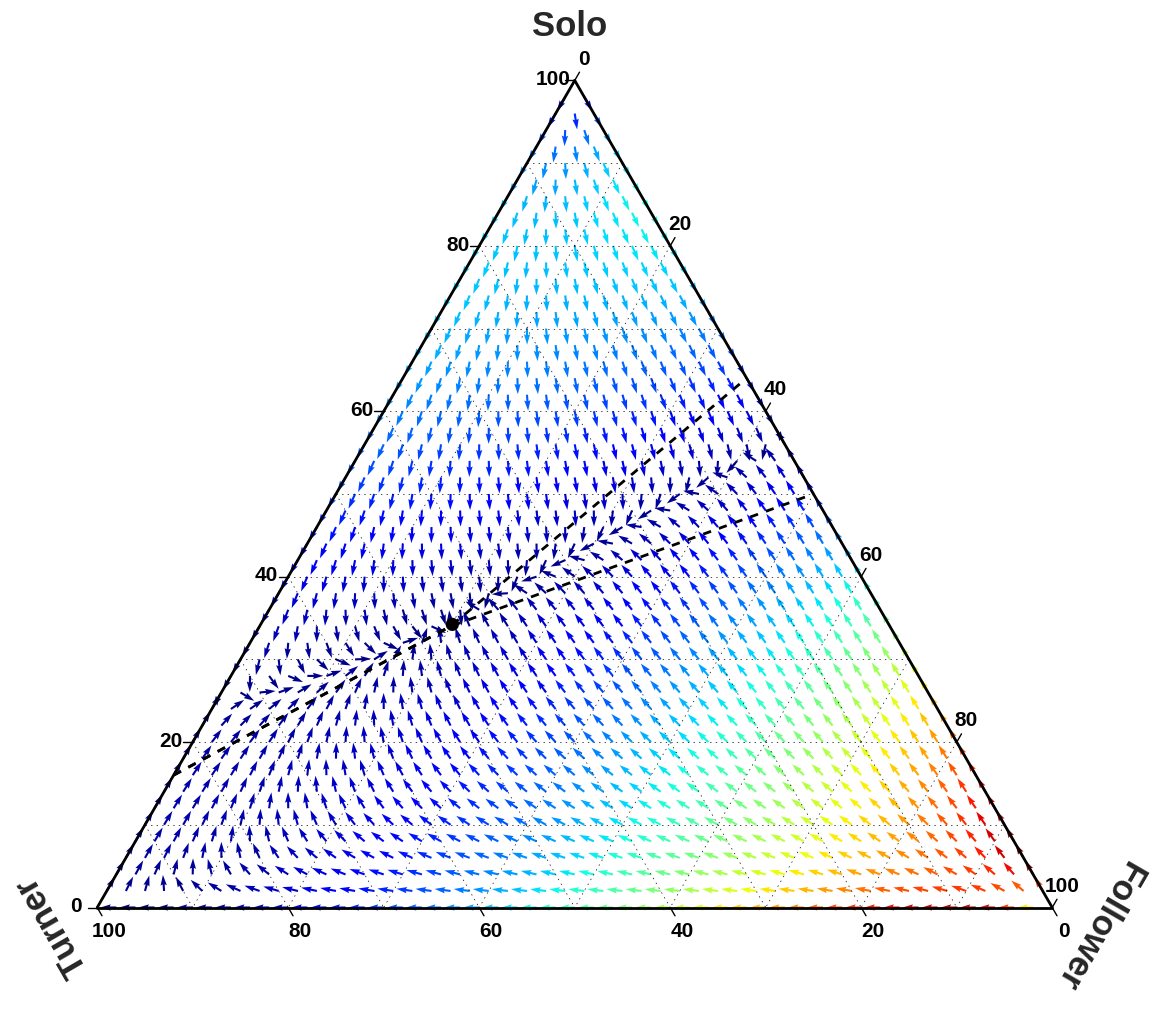
\includegraphics[scale=0.26]{fig/ArticleRob2/ExpectationsVectorsNormalized.png}}
          \end{subfigure}
          \begin{subfigure}[]
            {\label{fig:expectationsScatter} 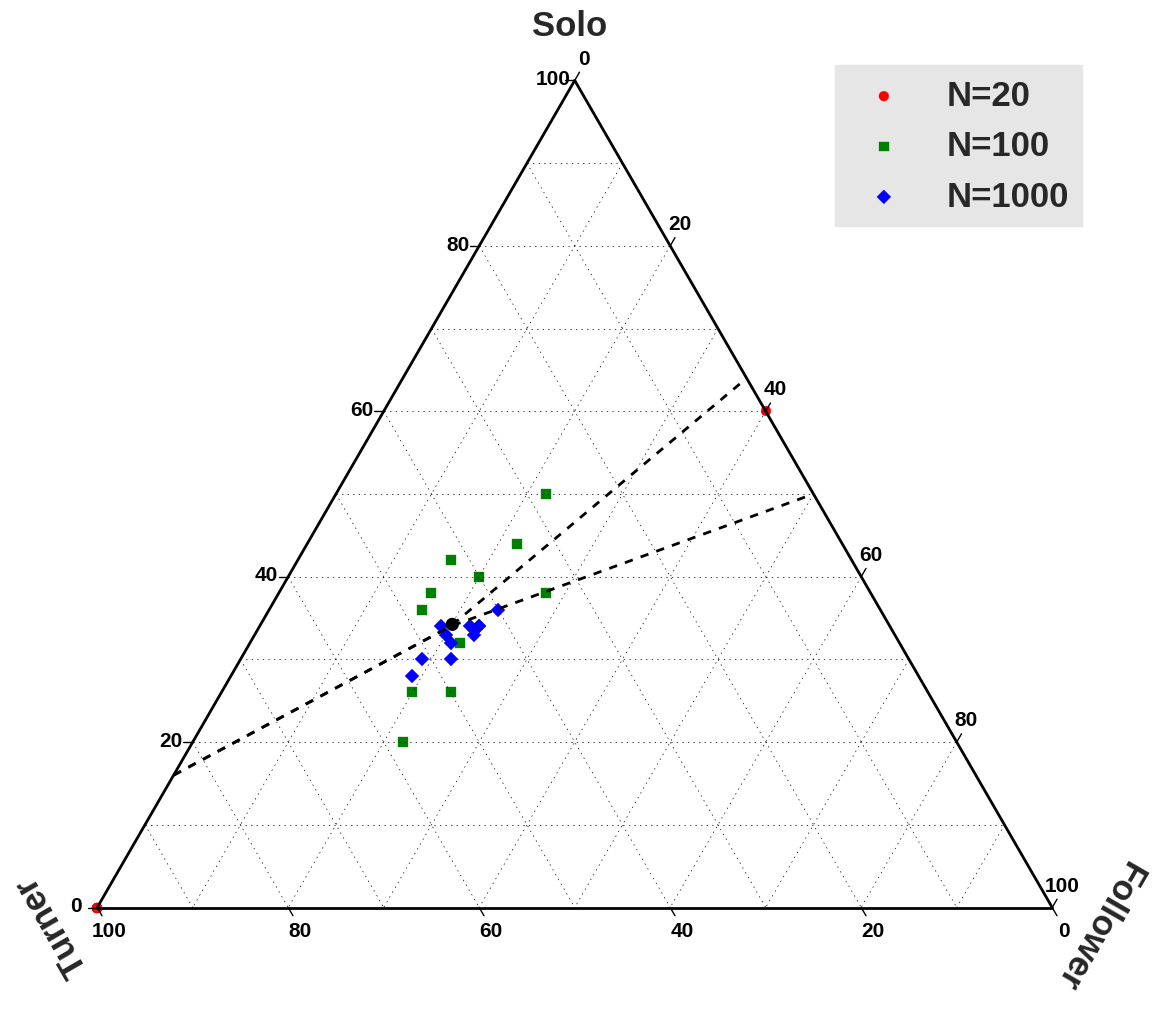
\includegraphics[scale=0.26]{fig/ArticleRob2/ExpectationsScatter.png}}
          \end{subfigure}
          \caption{\textbf{Vector field of the gradient of phenotypes' proportions and proportions of phenotypes at last generation of evolution.} {\em (a)}~Vector field of the gradient of phenotypes' proportions in an infinite population. The strength of variation is indicated by the color of the arrow. {\em (b)}~Repartition of phenotypes at the last generation of evolution for all three population sizes. Evolution lasted $1500$ generations and results were replicated across $11$ independent simulations. The initial population was entirely composed of \emph{solo} individuals.}
          \label{fig:ternary}
      \end{figure}

      Figure~\ref{fig:expectationsScatter} shows the final repartition of phenotypes after $1500$ generation of evolution for \(N=20\), \(N=100\) and \(N=1000\) in $11$ independent replicates. We can see that when increasing population size we also increase the probability that an equilibrium where the three phenotypes coexist is reached. We actually observe that the repartition of phenotypes at the last generation of evolution gets closer to the predicted equilibrium as population size increases. This implies that when population size increases, the effects of stochastic selection in a finite population decreases. Therefore the probability to lose particular phenotypes due to stochasticity is mitigated: population size is essential to the maintenance of specialists.


  \subsection{Key Properties for Evolving Heterogeneous Behaviours}

    From the previous Sections, we can deduce two key properties for the successful evolution of genotypic polymorphism. First, we showed that population size needs to be large enough in order to decrease the probability that heterogeneity could be lost during the evolutionary time. From this observation, we hypothesize that \textit{individuals need to be protected against the stochastic effects of selection}. Second, we previously saw that one key reason for the invasion of \emph{turner} individuals is that they perform quite well when paired together, even though they do not yield the best results. In other words, evolutionary dynamics does not necessarily lead to the best pairing in terms of performance, but to the most stable equilibrium between phenotypes.
  % while a pair of two \emph{followers} will perform badly and a pair with a \emph{solo} and a \emph{follower} fare better than any other. 
  From this observation, we hypothesize that \textit{the manner in which groups of interacting robots are formed is essential} for achieving an efficient specialisation.

    In order to test these hypotheses we design a last experiment where we diverge from the initial problem and now coevolve two separate populations. In this coevolution algorithm, each individual of one population is always evaluated against an individual of the other population ($5$ times as in previous experiments). Then, each population separately undergoes selection under an elitist \((10+10)\) selection method to create the population of the next generation (which means that each population's size is $20$). We conducted $11$ independent replicates which lasted $90000$ evaluations each. The populations were initially constituted of random individuals.

    \begin{table}[hbtp]
      \center{
        \begin{tabular}{cccc}
          \hline
          \textbf{\# L/F} & \textbf{\# Turning} & \textbf{\# NC} & \textbf{Total}\\ 
          \textbf{Strat.} & \textbf{Strat.} & \textbf{Strat.} & \\ 
          \hline
          11 & 0 & 0 & \textbf{11}\\
          \hline
        \end{tabular}
      }
      \caption{\textbf{Strategies evolved by the best individuals when coevolving two populations.} Repartition of the different strategies adopted by the best individuals at the last evaluation in each of the $11$ replicates. We indicate in each cell the number of simulations where a particular strategy evolved. Two populations were coevolved under elitist selection and the individuals' genotype values were initially random. In the table "L/F" stands for leader/follower and "NC" for "Non-Cooperative".}
      \label{tab:coevoStrategies}
    \end{table}

    We show (Table~\ref{tab:coevoStrategies}) that when using coevolution, we always evolve specialists in every replicates. Moreover, this algorithm is highly stable as the heterogeneous behaviours that emerged were never lost during evolution in every replicates. This means that coevolution is highly efficient both for the bootstrap of a leader/follower strategy and its maintenance throughout evolution. Regarding our hypotheses, we can check that the coevolution algorithm respects both of them. Firstly, as population are separatly coevolved, this algorithm is not sensible to the stochastic effects of small population size. Thus we ensure that the populations are highly protected against the disappearance of specialists. Secondly, we enforce a very specific pairing between individuals. Indeed individuals inside the same population are never partnered with one another. In this particular setup, this means that \emph{followers} end up being always paired with \emph{solo} individuals. As \emph{turners} then possesses no fitness benefit over the other phenotypes, their invasion will be prevented. The question is open as to how to endow an algorithm working on a single population with such properties.

  \subsection{Discussion and Conclusions}
  \label{sec:discussion}
    In this paper, we investigated the evolution of specialisation through a leader/follower strategy in a cooperative foraging task. Our goal was to reveal the difficulties that arise when trying to evolve genotypic polymorphism in a single population. To that end, we mainly studied the dynamics of evolution with two different selection methods: an \((\mu + \lambda)\) selection scheme and a fitness-proportionate selection scheme.

    We first showed that the long term evolution of a leader/follower strategy was nearly impossible with an elitist selection. However bootstrapping specialists was not a problem as we observed that they frequently emerged (and disappeared) during evolution. The major obstacle was rather to maintain heterogeneity over evolutionary time. Indeed, even when adding efficient \emph{followers} to a population of \emph{solo} individuals (i.e. \emph{leaders}) to force the adoption of a leader/follower strategy, specialists couldn't be maintained. In comparison, the properties shown by the fitness-proportionate algorithm were quite the opposite. While it was almost not capable of evolving a leader/follower strategy (nor any other cooperative strategy), the fitness-proportionate selection demonstrated high stability. It was therefore capable of maintaining specialists when present. We thus revealed two critical properties for evolving heterogeneous behaviours in a single population: \emph{bootstrapping} these behaviours and \emph{maintaining} them throughout evolution.

    We then ran computational analyses and showed that while a pair of \emph{turners} is indeed less efficient w.r.t. payoff than a pair of \emph{leader} and \emph{follower}, it is a lot more efficient than a pair of \emph{leaders} or a pair of \emph{followers}. As a result, these individuals can easily invade part of the population. Moreover, we also showed that the maintenance of specialists was very sensible to population size. Stochasticity in the selection process can indeed affect the stability of heterogeneity. Finally, a coevolution algorithm, which we showed to be always successful in evolving heterogeneous behaviours, solved both of these two problems with (1) \emph{specific partners selection} as pairs were constituted of individuals from different populations and (2) \emph{protection} of the behaviours evolved by applying selection separately on the two populations. While this coevolutionary algorithm is not capable (by design) of displaying genotypic polymorphism in a single population, it is sufficient to test and validate our hypotheses regarding the necessary properties for evolving efficient cooperative behaviours. Of course, the actual design of an algorithm using only one population to evolve heterogeneous individuals remains to be proposed.
    
    This raises several interesting perspectives on how to solve this problem. First, niche protection could prevent the disappearance of the efficient but unstable leader/follower strategy. As a matter of fact, coevolution is akin to a particular type of niches protection with $2$ niches. However, we intend to investigate how we could implement such mechanism without specifying the explicit number nor the organization of the niches. Rewarding diversity~\cite{Lehman2008} is also known as an effective way to protect novel behaviours and could be another promising direction. In particular, a multiobjective algorithm on performance and diversity~\cite{Doncieux2014}, by rewarding genotypic and phenotypic diversity, may protect evolved specialists.

    Secondly, we showed that because partners were chosen randomly among the population, it created the opportunity for a "parasitic" strategy to invade. An interesting direction for future work could be to investigate restrictions in the choice of partners. For example it would be compelling to investigate how the individuals could evolve to select their partner based on genotypic or phenotypic information.
  